\chapter{Análisis y resultados}
En este capítulo se van a discutir los resultados obtenidos tras realizar los experimentos descritos en el capítulo anterior. Se mostrarán gráficas que ilustren la curva de convergencia de los algoritmos en algunos conjunto de datos, para cada clasificador (kNN y SVC) y en cada versión del algoritmo, es decir, original y versión binaria. Junto a eso también se han elaborado una gráficas de ``cajas y bigotes'' o \textit{boxplots} que ilustran no solo los mejores resultados, sino su robustez y estabilidad tras varias iteraciones. \\[6pt]
Además se mostrarán tablas y gráficas de los ranking obtenidos en versión binaria y en versión continua para cada clasificador tras hacer la media de los resultados en todos los conjuntos de datos.\\[6pt]
Por último, los resultados vendrán expuestos en forma de tabla junto a las métricas correspondientes, de forma que se facilite el análisis de los algoritmos, de las versiones reales y continuas y de los clasificadores usados.\\[6pt]
También ser realizarán análisis estadísticos de los resultados obtenidos utilizando como herramienta la página web \textbf{TACOlab}~\cite{taco_website}, facilitada por el tutor del proyecto, de forma que se puedan hacer los mejores y más robustos tests de forma automática y sencilla.\\[6pt]
Como detalle a tener en cuenta, se ha añadido en las comparaciones un optimizador al que se le ha llamado ``Dummy'', debido a su naturaleza totalmente aleatorio y sin criterio alguno. Se añade como algoritmo de referencia, ninguna otra metaheurística debería ser peor que esta en promedio. En caso contrario podría decirse que el algoritmo en cuestión está mal diseñado.\\[6pt]
Pese a que se dividirán los análisis entre binario y continuo, las versiones discretas se escribirán con la letra \textit{b} delante. Por ejemplo, el algoritmo \textbf{FA} en binario sería \textbf{bFA}.

\section{Binario}
En esta sección se discutirán y analizarán los resultados para las metaheurísticas de codificación binaria o discreta. Estas versiones tienen un enfoque del problema distinto al de las reales, pues codifican cada característica con un $0$ o un $1$, o lo que es lo mismo, descartan características. Dada su naturaleza, cabría pensar que son los algoritmos más específicos que podrían usarse para el problema se selección de características.

\subsection{General}
En esta sub-sección se presentarán los resultados generales obtenidos con las metaheurísticas binarias. Esto permitirá una visión más amplia de su desempeño y proporcionará intuiciones iniciales sobre la efectividad de cada algoritmo en distintos contextos.

\begin{figure}[htp]
    \centering
    \begin{subfigure}[htp]{1\textwidth}
        \includegraphics[width=\textwidth]{imagenes/fitness_charts/img/binary/rankings_knn_avg.png}
        \caption{Ranking por fitness para knn - binario}
        \label{fig:ranking_knn}
    \end{subfigure}
    \begin{subfigure}[htp]{1\textwidth}
        \includegraphics[width=\textwidth]{imagenes/fitness_charts/img/binary/rankings_svc_avg.png}
        \caption{Ranking por fitness para svc - binario}
        \label{fig:ranking_svc}
    \end{subfigure}
    \caption{Rankings para fitness - binario}
\end{figure}

Como ya se aclaró en capítulos anteriores, para obtener estos resultados se han ejecutado $10$ veces cada algoritmo en cada conjunto de datos. Se muestran los resultados generales de rankings en para \textbf{SVC} y \textbf{kNN} en \ref{fig:ranking_knn} y \ref{fig:ranking_svc}, respectivamente.\\[6pt]
Como puede apreciarse en los rankings mencionados, los algoritmos con mejor rendimiento son \textbf{bGWO}, \textbf{bPSO}, \textbf{bCS} y \textbf{GA}. En concreto, \textbf{bGWO} obtiene una diferencia muy notable con respecto al resto de los algoritmos.\\[6pt]
Los peores son \textbf{bABCO}, \textbf{bGOA} y \textbf{bDA}. Además lo son con una puntuación que los diferencia mucho del los algoritmos con un rendimiento medio, sobre todo \textbf{bABCO}.\\[6pt]
También es apreciable que los mejores algoritmos producen mejores resultados de media en \textbf{SVC} que en \textbf{kNN}, aunque los resultados de todo el conjunto de algoritmos parecen más estables en \textbf{kNN}.

\subsection{Variabilidad}

\begin{figure}[htp]
    \centering
    \begin{subfigure}[htp]{0.5\textwidth}
        \includegraphics[width=\textwidth]{imagenes/fitness_charts/results/binary/ionosphere/optimizer_boxplot_fitness_knn_b.png}
        \caption{ionosphere}
        \label{fig:boxplot_ionosphere}
    \end{subfigure}

    \begin{subfigure}[htp]{0.5\textwidth}
        \includegraphics[width=\textwidth]{imagenes/fitness_charts/results/binary/wdbc/optimizer_boxplot_fitness_knn_b.png}
        \caption{wdbc}
        \label{fig:boxplot_wdbc}
    \end{subfigure}

    \begin{subfigure}[htp]{0.5\textwidth}
        \includegraphics[width=\textwidth]{imagenes/fitness_charts/results/binary/diabetes/optimizer_boxplot_fitness_knn_b.png}
        \caption{diabetes}
        \label{fig:boxplot_diabetes}
    \end{subfigure}

    \begin{subfigure}[htp]{0.5\textwidth}
        \includegraphics[width=\textwidth]{imagenes/fitness_charts/results/binary/parkinsons/optimizer_boxplot_fitness_knn_b.png}
        \caption{parkinsons}
        \label{fig:boxplot_parkinsons}
    \end{subfigure}

    \caption{\textit{Boxplots} para kNN - binario}
    \label{fig:boxplot_knn-bin}
\end{figure}

Se muestran algunos de los resultados obtenidos con los algoritmos binarios en \ref{fig:boxplot_ionosphere}, \ref{fig:boxplot_wdbc}, \ref{fig:boxplot_diabetes} y \ref{fig:boxplot_parkinsons} con el clasificador \textbf{kNN}. Obviamente, no es posible incluir gráficas para todas las combinaciones posibles sin saturar el capítulo; para ello, se remite al lector al capítulo de apéndices.\\[6pt]
Se puede observar que la mayoría de los algoritmos obtienen resultados bastante buenos en los distintos conjuntos de datos, considerándose los valores de fitness suficientemente buenos para considerarlos soluciones de calidad, obviamente considerando cada problema por separado, con las características de cada uno. Es importante destacar que no todos los conjuntos de datos presentan la misma dificultad, ya que distintos tipos de problemas presentan diferentes desafíos. En particular, se puede notar que los algoritmos aplicados al conjunto de datos \textit{ionosphere} (figura \ref{fig:boxplot_ionosphere}) muestran menos variabilidad en sus valores de fitness, reflejándose en una desviación estándar menor en comparación con los resultados de \textit{diabetes} (figura \ref{fig:boxplot_diabetes}) o \textit{parkinsons} (figura \ref{fig:boxplot_parkinsons}). Con ello, queda reflejado como a los algoritmos les cuesta menos optimizar ciertos problemas y suelen ser más estables en estos. Esto puede deberse muchos factores, por ejemplo, mayor cantidad de mínimos locales en algunos problemas en comparación a otros.\\[6pt]
También se pueden identificar ciertos algoritmos que parecen tener un mejor desempeño en general. Por ejemplo, algoritmos como \textbf{bGWO} y \textbf{bPSO} tienden a obtener resultados muy buenos y poco variantes, mientras que otros como \textbf{ACO} y \textbf{bABCO} parecen ser menos efectivos en los conjuntos de datos analizados.\\[6pt]
Pese a ello, se percibe una variabilidad de los resultados en \textit{fitness} bastante similar en todos los algoritmos usados. Donde un algoritmo es robusto en cuanto a variabilidad, en otro no lo es. Esto se observa en todos los problemas.

\subsection{Fitness}
Se procede a comparar y analizar los distintos algoritmos basándonos en la métrica de \textit{fitness}. Como se explica en la ecuación \ref{eq:fitness}, este valor está compuesto por otras dos métricas a tener en cuenta, la precisión o \textit{accuracy} y el ratio de reducción de características. La métrica de \textit{fitness} es el marcador más importante para comprobar la calidad de un algoritmo. Pese a ello, más tarde se analizarán ambas métricas que lo componen por separado, pues es interesante obtener una visión más precisa de los resultados.\\[6pt]
Debe tenerse en cuenta que, al estar compuesto el \textit{fitness} en un $90\%$ por el \textit{accuracy}, ambas métricas estarán altamente relacionadas entre sí en la gran mayoría de los casos.\\[6pt]
Como puede observarse en la tabla \ref{tab:fitness_svc}, los algoritmos que consiguen mejores resultados son \textbf{ACO}, \textbf{bGWO}, \textbf{bPSO}, \textbf{bFA}, \textbf{bDE}, \textbf{bGA}, \textbf{bCS} y \textbf{bWOA} con el clasificador \textbf{SVC}. Los más destacables en cuanto al número de veces que estos se repiten por ser los mejores por \textit{dataset} son \textbf{bCS}, \textbf{ACO}, \textbf{bDE} y \textbf{bGWO} \ref{tab:n-best-fitness_combined}. Puede verse que en \textbf{SVC} los resultados son más discriminativos y se reparten menos los mejores resultados entre el conjunto completo de algoritmos.

\begin{table}[htp]
    \centering
    \begin{tabular}{ccc}
        \toprule
        Algoritmo     & N veces mejor (knn) & N veces mejor (svc) \\
        \midrule
        \textbf{bCS}  & 2                   & 4                   \\
        \textbf{ACO}  & 1                   & 3                   \\
        \textbf{bDE}  & 2                   & 2                   \\
        \textbf{bGWO} & 3                   & 2                   \\
        \bottomrule
    \end{tabular}
    \caption{Algoritmos con más veces mejor resultados - knn y svc - binario}
    \label{tab:n-best-fitness_combined}
\end{table}

\subsubsection{Mejor vs Peor}
Como se puede observar en \ref{fig:ranking_knn} y en \ref{fig:ranking_svc}, el algoritmo con mejor puntuación es \textbf{bGWO} y el peor \textbf{bABCO} (se puede ver también su valor en los rankings de las tablas en el apéndice: \ref{tab:ranking_fitness_bin_svc}, \ref{tab:ranking_fitness_bin_knn}). \\[6pt]
En las figuras de \ref{fig:convergencia_svc_2} y \ref{fig:convergencia_svc_1} se aprecia como \textbf{bABCO} muestra rendimientos muy buenos en según que conjunto de datos. Por ejemplo, en \textit{yeast} o en \textit{sonar}, el algoritmo obtiene resultados muy decentes y competitivos siendo estos dos conjuntos de datos de los más complicados de la selección, por convergencia y número de características. Pese a ello, en conjunto, no consigue superar al resto.\\[6pt]
En cambio \textbf{bGWO} parece un adaptarse bien a todos los problemas seleccionados sin excepción. Es capaz de obtener el mínimo, en el valor \textit{fitness} de evaluación durante el entrenamiento, en casi todos los \textit{datasets}.

\begin{table}[htp]
    \centering
    \begin{tabular}{lllll}
        \toprule
        {}    & Original  & Holm           & Hommel         & Hochberg       \\
        \midrule
        dummy & 6.104E-05 & \textbf{0.001} & \textbf{0.001} & \textbf{0.001} \\
        abco  & 0.003     & \textbf{0.029} & \textbf{0.029} & \textbf{0.029} \\
        da    & 0.005     & 0.054          & 0.051          & 0.054          \\
        goa   & 0.010     & 0.092          & 0.082          & 0.092          \\
        fa    & 0.022     & 0.172          & 0.106          & 0.172          \\
        de    & 0.026     & 0.179          & 0.106          & 0.179          \\
        ga    & 0.038     & 0.230          & 0.127          & 0.191          \\
        ba    & 0.055     & 0.277          & 0.166          & 0.191          \\
        aco   & 0.055     & 0.277          & 0.166          & 0.191          \\
        woa   & 0.064     & 0.277          & 0.191          & 0.191          \\
        cs    & 0.135     & 0.277          & 0.271          & 0.271          \\
        pso   & 0.346     & 0.346          & 0.346          & 0.346          \\
        \bottomrule
    \end{tabular}
    \caption{P-valores del bGWO vs el resto - knn - binario}
    \label{tab:p-values_gwo_vs_rest_knn}
\end{table}

\begin{table}[htp]
    \centering
    \begin{tabular}{lllll}
        \toprule
        {}    & Original  & Holm           & Hommel         & Hochberg       \\
        \midrule
        dummy & 3.052E-04 & \textbf{0.004} & \textbf{0.004} & \textbf{0.004} \\
        abco  & 0.002     & \textbf{0.024} & \textbf{0.022} & \textbf{0.024} \\
        ba    & 0.004     & \textbf{0.043} & \textbf{0.037} & \textbf{0.043} \\
        da    & 0.005     & \textbf{0.048} & \textbf{0.043} & \textbf{0.048} \\
        goa   & 0.008     & 0.066          & 0.066          & 0.066          \\
        woa   & 0.073     & 0.514          & 0.367          & 0.514          \\
        de    & 0.109     & 0.656          & 0.547          & 0.599          \\
        fa    & 0.121     & 0.656          & 0.599          & 0.599          \\
        ga    & 0.252     & 1.000          & 0.599          & 0.599          \\
        cs    & 0.364     & 1.000          & 0.599          & 0.599          \\
        aco   & 0.490     & 1.000          & 0.599          & 0.599          \\
        pso   & 0.599     & 1.000          & 0.599          & 0.599          \\
        \bottomrule
    \end{tabular}
    \caption{P-valores del bGWO vs el resto - svc - binario}
    \label{tab:p-values_gwo_vs_rest_svc}
\end{table}

Se procede a hacer una comparativa estadística mediante la prueba de \textit{Wilcoxon} y el test post hoc de \textit{Holm} para determinar las diferencias significativas entre el mejor algoritmo (\textbf{bGWO}) y el resto. Los resultados, presentados en las tablas \ref{tab:p-values_gwo_vs_rest_knn} y \ref{tab:p-values_gwo_vs_rest_svc}, muestran los p-valores originales y ajustados, lo que nos permite identificar cuáles de las diferencias observadas son estadísticamente significativas con un error corregido. Este análisis es crucial para validar los resultados y asegurar que las conclusiones obtenidas no sean producto del azar, proporcionando una base sólida para afirmar la superioridad de \textbf{bGWO} frente a los demás algoritmos en los conjuntos de datos evaluados, en frente al peor de ellos.\\[6pt]

Si bien no se observan diferencias significativas sobre la mayoría de algoritmos, sí sobre el peor (\textbf{bABCO}) usando \textbf{kNN}. Tanto en la versión que utiliza el clasificador \textbf{SVC} como en \textbf{kNN} se obtienen resultados suficientemente significativos como para poder considerar que los resultados de \textbf{bGWO} frente a los de \textbf{bABCO} no son producto del azar. Por tanto, utilizando un valor crítico de $\alpha=0.05$ se puede rechazar la hipótesis nula. Esto no solo ocurre con \textbf{bABCO} en los resultados de \textbf{SVC}, sino que también con \textbf{bBA} y \textbf{bDA}. Por ello se puede afirmar que \textbf{bGWO} en este último clasificador es mejor, con un respaldo estadístico, frente a esos algoritmos también.

\subsubsection{Clásicos vs Modernos}
Los algoritmos clásicos de optimización como el \textbf{bPSO}, \textbf{bGA} o \textbf{bDE} han demostrado ser extremadamente efectivos en una amplia gama de problemas. Su capacidad para explorar y explotar el espacio de búsqueda ha llevado a soluciones de alta calidad en diversas aplicaciones, desde la ingeniería hasta la economía. Estos métodos son conocidos por su robustez, simplicidad y eficacia, lo que los convierte en herramientas valiosas.\\[6pt]
Sin embargo, en los últimos años, han surgido nuevos algoritmos de optimización que prometen mejorar aún más estos resultados. Algoritmos como el \textbf{bWOA}, \textbf{bGWO} y \textbf{bCS}, aunque este último es de hecho bastante antiguo, han sido diseñados para abordar algunas de las limitaciones de los métodos clásicos, como la convergencia prematura y la exploración insuficiente del espacio de búsqueda. Estos algoritmos modernos incorporan nuevas estrategias y mecanismos de búsqueda inspirados en la naturaleza, que buscan mejorar la eficiencia y la precisión de las soluciones obtenidas.\\[6pt]

Los rankings han sido creados basándose en los valores \textit{fitness} de los algoritmos para todos los conjuntos de datos. De forma visual es capaz de verse de un vistazo aquellos más versátiles, los que mejor se han comportado en distintos escenarios. En los rankings que se pueden observar en las gráficas \ref{fig:ranking_knn} para \textbf{kNN} y en \ref{fig:ranking_svc} para \textbf{SVC} puede verse como el mejor algoritmo es el \textbf{bGWO}, el algoritmo de los lobos grises, considerado como moderno. Le siguen algoritmos como \textbf{bPSO}, \textbf{bCS} y \textbf{bGA}.\\[6pt]

El \textbf{bPSO}, a pesar de ser uno de los algoritmos más antiguos en la optimización metaheurística, sigue manteniendo una posición destacada en los rankings. Estos hechos junto a su simplicidad y efectividad en la convergencia hacia soluciones óptimas, hacen ver que \textbf{bPSO} sigue siendo una opción muy interesante, incluso en problemas de tipo binario como la selección de características, escenario para los que \textbf{bPSO} no fue diseñado. Esto hace de esta metaheurística una opción que parece sugerir mucha robustez.\\[6pt]

El \textbf{bCS}, basado en el comportamiento de anidación de ciertos pájaros, también se muestra como una opción fuerte, compitiendo por el podio con \textbf{bGA}.\\[6pt]

Finalmente, el \textbf{bGA}, uno de los algoritmos más estudiados y aplicados en el ámbito de la optimización, sigue siendo relevante. Su capacidad para encontrar soluciones óptimas a través de mecanismos inspirados en la evolución natural, como la selección, el cruce y la mutación, le permite abordar una amplia gama de problemas con éxito. Además, este algoritmo al ser inicialmente pensado para aplicarse en dominios de codificación discreta, hace de esta metaheurística una opción muy interesante y robusta en el problema de selección de características, además de llevar años siendo aplicado con éxito en otros dominios.\\[6pt]

Es visible que algunas de estas nuevas propuestas son muy potentes, llegando a mejorar en la propuesta binaria en comparación a algoritmos clásicos que llevan tiempo en la escena como las opciones \textit{de facto}. Pese a ello, el grueso de los algoritmos comparados son opciones modernas, y muchos de estos algoritmos clásicos obtienen mejores resultados que la mayoría de este reciente grupo. De los cinco mejores, tres de ellos son clásicos, lo cual es más impresionante si se considera que hay un desbalance en número de \textit{clásicos vs modernos}. \textbf{bDE} es otro algoritmo asentado, que es capaz de clasificar en posiciones medias de \textit{fitness}.\\[6pt]

Por tanto, los clásicos siguen siendo una opción muy potente e interesante. Pese a desarrollarse nuevos algoritmos, estos siguen obteniendo soluciones de alta calidad.


\subsection{Clasificación y reducción}
Como se ha mencionado al principio de la anterior sección y como se explica en la fórmula \ref{eq:fitness}, el \textit{fitness} está compuesto por las métricas de \textit{accuracy} en la clasificación y por el ratio de reducción de las características. Con ello se intenta reducir tantas características como sea posible, manteniendo un valor lo más alto posible de precisión.\\[6pt]
Con estos aspectos aclarados, en esta sección se analizarán los algoritmos desde la perspectiva individual de cada una de las métricas que componen la función \textit{fitness}. De esta manera, se proveerá información de cuál o cuáles algoritmos son los mejores para cada una de las métricas.\\[6pt]
Esta visión es interesante ya que, los pesos fijados por el autor para cada métrica son los estándar en la mayoría de artículos, pero es posible que en otros problemas sea necesario ajustarlos a las necesidades del mismo. Por tanto si se conocen las características de los diferentes algoritmos para cada métrica por separado, se obtendrá un conocimiento que proporcionará un uso de los mismos más flexible.

\subsubsection{Mejor vs Resto}
La metaheurística \textbf{ACO} es sin lugar a dudas la mejor en reducción de características (\ref{tab:ranking_sel_rate_bin_knn}, \ref{tab:ranking_sel_rate_bin_svc}) y a su vez, la peor en precisión según los rankings (\ref{tab:ranking_accuracy_bin_knn}, \ref{tab:ranking_accuracy_bin_svc}).
Un ejemplo de esto es en el conjunto de datos de \textit{ionosphere}. Se puede observar como el segundo algoritmo que más reduce, que es \textbf{bGWO}, obtiene una reducción media del $74\%$, mientras que el \textbf{ACO} obtiene una reducción media del $91.5\%$, con tan solo una diferencia de $4.6\%$ en precisión a favor de \textbf{bGWO}~\ref{tab:bin_red_acc_all}. \\[6pt]
Si bien es cierto que su precisión no es de las mejores, podría considerarse aceptable en muchos casos. Teniendo ese aspecto en cuenta, añadido a que es capaz de reducir características a un nivel muy significativo con respecto al resto de algoritmos, \textbf{ACO} se presenta como un algoritmo muy interesante para aquellos problemas en los que se pueda permitir cierto nivel de error en la precisión, pero en cambio, sea crucial una compresión del tamaño del modelo o un tiempo den entrenamiento corto.\\[6pt]

Los mejores algoritmos en \textit{accuracy} son \textbf{bCS} y \textbf{bGWO} como puede observarse en las tablas \ref{tab:ranking_accuracy_bin_knn} y \ref{tab:ranking_accuracy_bin_svc}, mientras que el peor, como se ha comentado anteriormente, es el \textbf{ACO}. Si bien es cierto que \textbf{bGWO} empata en \textbf{kNN} con \textbf{bBA}, este no se ha considerado como mejor por obtener un resultado peor en \textbf{SVC} mientras que \textbf{GWO} es bueno en ambos. Pese a ello, no hay grandes diferencias en los algoritmos del top.\\[6pt]

Si se comparan los p-valores~\ref{tab:p-values_aco_rest_bin_knn}, \ref{tab:p-values_aco_rest_bin_svc}, tras aplicar post hoc para mayor seguridad, de \textbf{ACO} con respecto al resto de algoritmos, se ve que claramente la mejora en reducción no se debe al azar de manera muy probable en todos los casos comparativos.

\begin{table}[htp]
    \centering
    \begin{tabular}{lllll}
        \toprule
        {}    & Original  & Holm           & Hommel         & Hochberg       \\
        \midrule
        dummy & 6.104E-05 & \textbf{0.001} & \textbf{0.001} & \textbf{0.001} \\
        fa    & 6.104E-05 & \textbf{0.001} & \textbf{0.001} & \textbf{0.001} \\
        goa   & 6.104E-05 & \textbf{0.001} & \textbf{0.001} & \textbf{0.001} \\
        abco  & 0.001     & \textbf{0.010} & \textbf{0.002} & \textbf{0.002} \\
        ba    & 0.001     & \textbf{0.010} & \textbf{0.002} & \textbf{0.002} \\
        cs    & 0.001     & \textbf{0.010} & \textbf{0.002} & \textbf{0.002} \\
        da    & 0.001     & \textbf{0.010} & \textbf{0.002} & \textbf{0.002} \\
        de    & 0.001     & \textbf{0.010} & \textbf{0.002} & \textbf{0.002} \\
        ga    & 0.001     & \textbf{0.010} & \textbf{0.002} & \textbf{0.002} \\
        pso   & 0.001     & \textbf{0.010} & \textbf{0.002} & \textbf{0.002} \\
        woa   & 0.001     & \textbf{0.010} & \textbf{0.002} & \textbf{0.002} \\
        gwo   & 0.002     & \textbf{0.010} & \textbf{0.002} & \textbf{0.002} \\
        \bottomrule
    \end{tabular}
    \caption{P-valores de ACO vs el resto - knn - binario}
    \label{tab:p-values_aco_rest_bin_knn}
\end{table}

\begin{table}[htp]
    \centering
    \begin{tabular}{lllll}
        \toprule
        {}    & Original  & Holm           & Hommel         & Hochberg       \\
        \midrule
        dummy & 6.104E-05 & \textbf{0.001} & \textbf{0.001} & \textbf{0.001} \\
        fa    & 6.104E-05 & \textbf{0.001} & \textbf{0.001} & \textbf{0.001} \\
        goa   & 6.104E-05 & \textbf{0.001} & \textbf{0.001} & \textbf{0.001} \\
        abco  & 0.001     & \textbf{0.010} & \textbf{0.001} & \textbf{0.001} \\
        ba    & 0.001     & \textbf{0.010} & \textbf{0.001} & \textbf{0.001} \\
        cs    & 0.001     & \textbf{0.010} & \textbf{0.001} & \textbf{0.001} \\
        da    & 0.001     & \textbf{0.010} & \textbf{0.001} & \textbf{0.001} \\
        de    & 0.001     & \textbf{0.010} & \textbf{0.001} & \textbf{0.001} \\
        ga    & 0.001     & \textbf{0.010} & \textbf{0.001} & \textbf{0.001} \\
        pso   & 0.001     & \textbf{0.010} & \textbf{0.001} & \textbf{0.001} \\
        woa   & 0.001     & \textbf{0.010} & \textbf{0.001} & \textbf{0.001} \\
        gwo   & 0.001     & \textbf{0.010} & \textbf{0.001} & \textbf{0.001} \\
        \bottomrule
    \end{tabular}
    \caption{P-valores de ACO vs el resto - svc - binario}
    \label{tab:p-values_aco_rest_bin_svc}
\end{table}

En cuanto a la clasificación, no se encuentran diferencias significativas entre los algoritmos, a excepción del \textbf{bCS} contra el \textbf{ACO}, el cual parece ser significativamente peor.

\subsubsection{Clásicos vs Modernos}
Se procede a comparar los algoritmos clásicos frente a los algoritmos modernos en cuanto a su capacidad clasificatoria, es decir, el valor de cada uno de ellos obtenido en \textit{accuracy}.\\[6pt]

En los rankings definidos en la tabla \ref{tab:ranking_accuracy_bin_knn} y en \ref{tab:ranking_accuracy_bin_svc}, el top de los mejores algoritmos está compuesto por los algoritmos \textbf{CS}, \textbf{FA}, \textbf{GWO}, \textbf{DE}, y \textbf{PSO} en \textbf{SVC}, y los algoritmos \textbf{WOA}, \textbf{BA}, \textbf{GWO}, \textbf{PSO}, y \textbf{FA} en \textbf{kNN}. El top de los peores algoritmos está compuesto, en cambio, por \textbf{GOA}, \textbf{ACO}, \textbf{DA}, y \textbf{GA} en \textbf{SVC}, y los algoritmos \textbf{ACO}, \textbf{DA}, \textbf{GOA}, y \textbf{GA} en \textbf{kNN}.\\[6pt]

Si bien es cierto que la mayoría en el top de mejores algoritmos en \textit{accuracy} son algoritmos modernos, los clásicos no se quedan atrás. En las comparaciones obtienen muy buenos resultados, no siendo los mejores y muy lejos de ser los peores. En los algoritmos modernos hay mayor diversidad en este punto. Hay unos pocos que destacan, pero el resto parecen verse superados en muchas ocasiones por los algoritmos clásicos.\\[6pt]

\begin{figure}[htp]
    \centering
    \begin{subfigure}[htp]{1\textwidth}
        \includegraphics[width=\textwidth]{imagenes/fitness_charts/img/binary/rankings_knn_selected_rate.png}
        \caption{Ranking por ratio de reducción para knn}
        \label{fig:ranking_knn_red}
    \end{subfigure}
    \begin{subfigure}[htp]{1\textwidth}
        \includegraphics[width=\textwidth]{imagenes/fitness_charts/img/binary/rankings_svc_selected_rate.png}
        \caption{Ranking por ratio de reducción para svc}
        \label{fig:ranking_svc_red}
    \end{subfigure}
    \caption{Rankings para reducción de características}
    \label{fig:rankings_red_bin}
\end{figure}

En cuanto a la reducción de características, se observa en los rankings \ref{fig:rankings_red_bin} como los mejores son algoritmos como \textbf{ACO}, \textbf{bGWO}, \textbf{GA} y \textbf{bPSO}. Incluso \textbf{bDE} es capaz de superar a varios modernos. El \textbf{bABCO}, sin embargo, parece obtener resultados pésimos, quedando el último en los rankings.\\[6pt]
Si se observan los p-valores obtenidos en las tablas \ref{tab:p-values_sel_ratio_bin_knn} y \ref{tab:p-values_sel_ratio_bin_svc}, y se agrupan los modernos y los clásicos, se obtienen los siguientes resultados:
\begin{itemize}
    \item \textbf{bPSO}: A excepción del \textbf{ACO} (el mejor), \textbf{bGWO} (segundo mejor) y \textbf{bGA}, es superior a todo el resto de algoritmos con una diferencia significativa más que suficiente tras corrección post hoc con el método \textit{Holms}.
    \item \textbf{ACO}: Es el mejor con diferencia significativa más que suficiente como para poder afirmar que este algoritmo es muy destacable en la reducción de características.
    \item \textbf{bGA}: Ocurre lo mismo que con \textbf{bPSO}. Pese a excepciones de algoritmos por encima suyo en el ranking, \textbf{bGA} es muy superior al resto de algoritmos, con diferencias muy notables y de nuevo significativas.
    \item \textbf{bDE}: Obtiene resultados muy buenos, pero en la media en comparación con todos.
    \item \textbf{bABCO}: El peor parado del grupo de los algoritmos clásicos. No parece ser una buena propuesta a la hora de reducir.
\end{itemize}

Dados estos resultados, los algoritmos clásicos salen muy bien parados en la reducción de características frente a los modernos. Si bien es cierto que hay dos algoritmos que destacan sobre el resto de los modernos (\textbf{bCS} y \textbf{bGWO}) en la reducción de características, los clásicos en conjunto, con excepción de \textbf{bABCO}, parecen una opción robusta y que, en combinación a sus resultados de precisión (\textit{accuracy}), son muy precisos a la hora de seleccionar características importantes. \\[6pt]

Por lo explicado, combinando los resultados analizados en \textit{accuracy} y en selección de características, se puede intuir que los algoritmos clásicos son muy eficientes en la reducción de características, superando a varios algoritmos modernos y además con una calidad en términos de \textit{accuracy} prácticamente idéntica.

\subsubsection{bWOA vs bGWO}
Dentro del conjunto de algoritmos analizados, hay ciertos pares que resultan interesantes por la semejanza algorítmica e inspirativa entre ambos. En esta sección, se compararán los algoritmos \textbf{bWOA} y \textbf{bGWO}. Ambos pertenecen a la categoría de algoritmos de optimización inspirados en la naturaleza y ambos se inspiran fuertemente en el comportamiento social y estrategias de caza de ciertos animales.\\[6pt]
Dentro del contexto de la caza, tanto \textbf{WOA} como \textbf{GWO} utilizan ecuaciones que simulan el rodeo de la presa, aunque con diferencias en la implementación y el comportamiento específico. A continuación se detallan los comportamientos de rodeo de la presa en la caza:
\begin{itemize}
    \item \textbf{bWOA}: La ballena ajusta su posición no solo moviéndose hacia la presa sino también rodeándola en un patrón circular, lo cual le permite cubrir más área y ajustar su aproximación con mayor precisión. La espiral seguida en la fórmula depende del parámetro de control $D$.
    \item \textbf{bGWO}: Los lobos rodean a la presa en grupos liderados por alfa, beta y delta. Al reducir la distancia a estas posiciones líderes, los lobos de menor rango simulan el cerco y convergen hacia la presa de manera cooperativa. El acercamiento utiliza un vector de coeficientes $A$ que decrece linealmente.
\end{itemize}

Ambos algoritmos por tanto, y pese a sus diferencias, comparten una naturaleza y comportamiento parecido a la hora buscar soluciones. Al comparar ambos resultados en \textit{accuracy}, se aprecia que estos no difieren de manera suficiente en su rendimiento como para poder rechazar la hipótesis nula. Véase en las tablas \ref{tab:p-values_accuracy_bin_knn}, \ref{tab:p-values_accuracy_bin_svc}.

\begin{figure}[htp]
    \centering
    \begin{subfigure}[htp]{0.45\textwidth}
        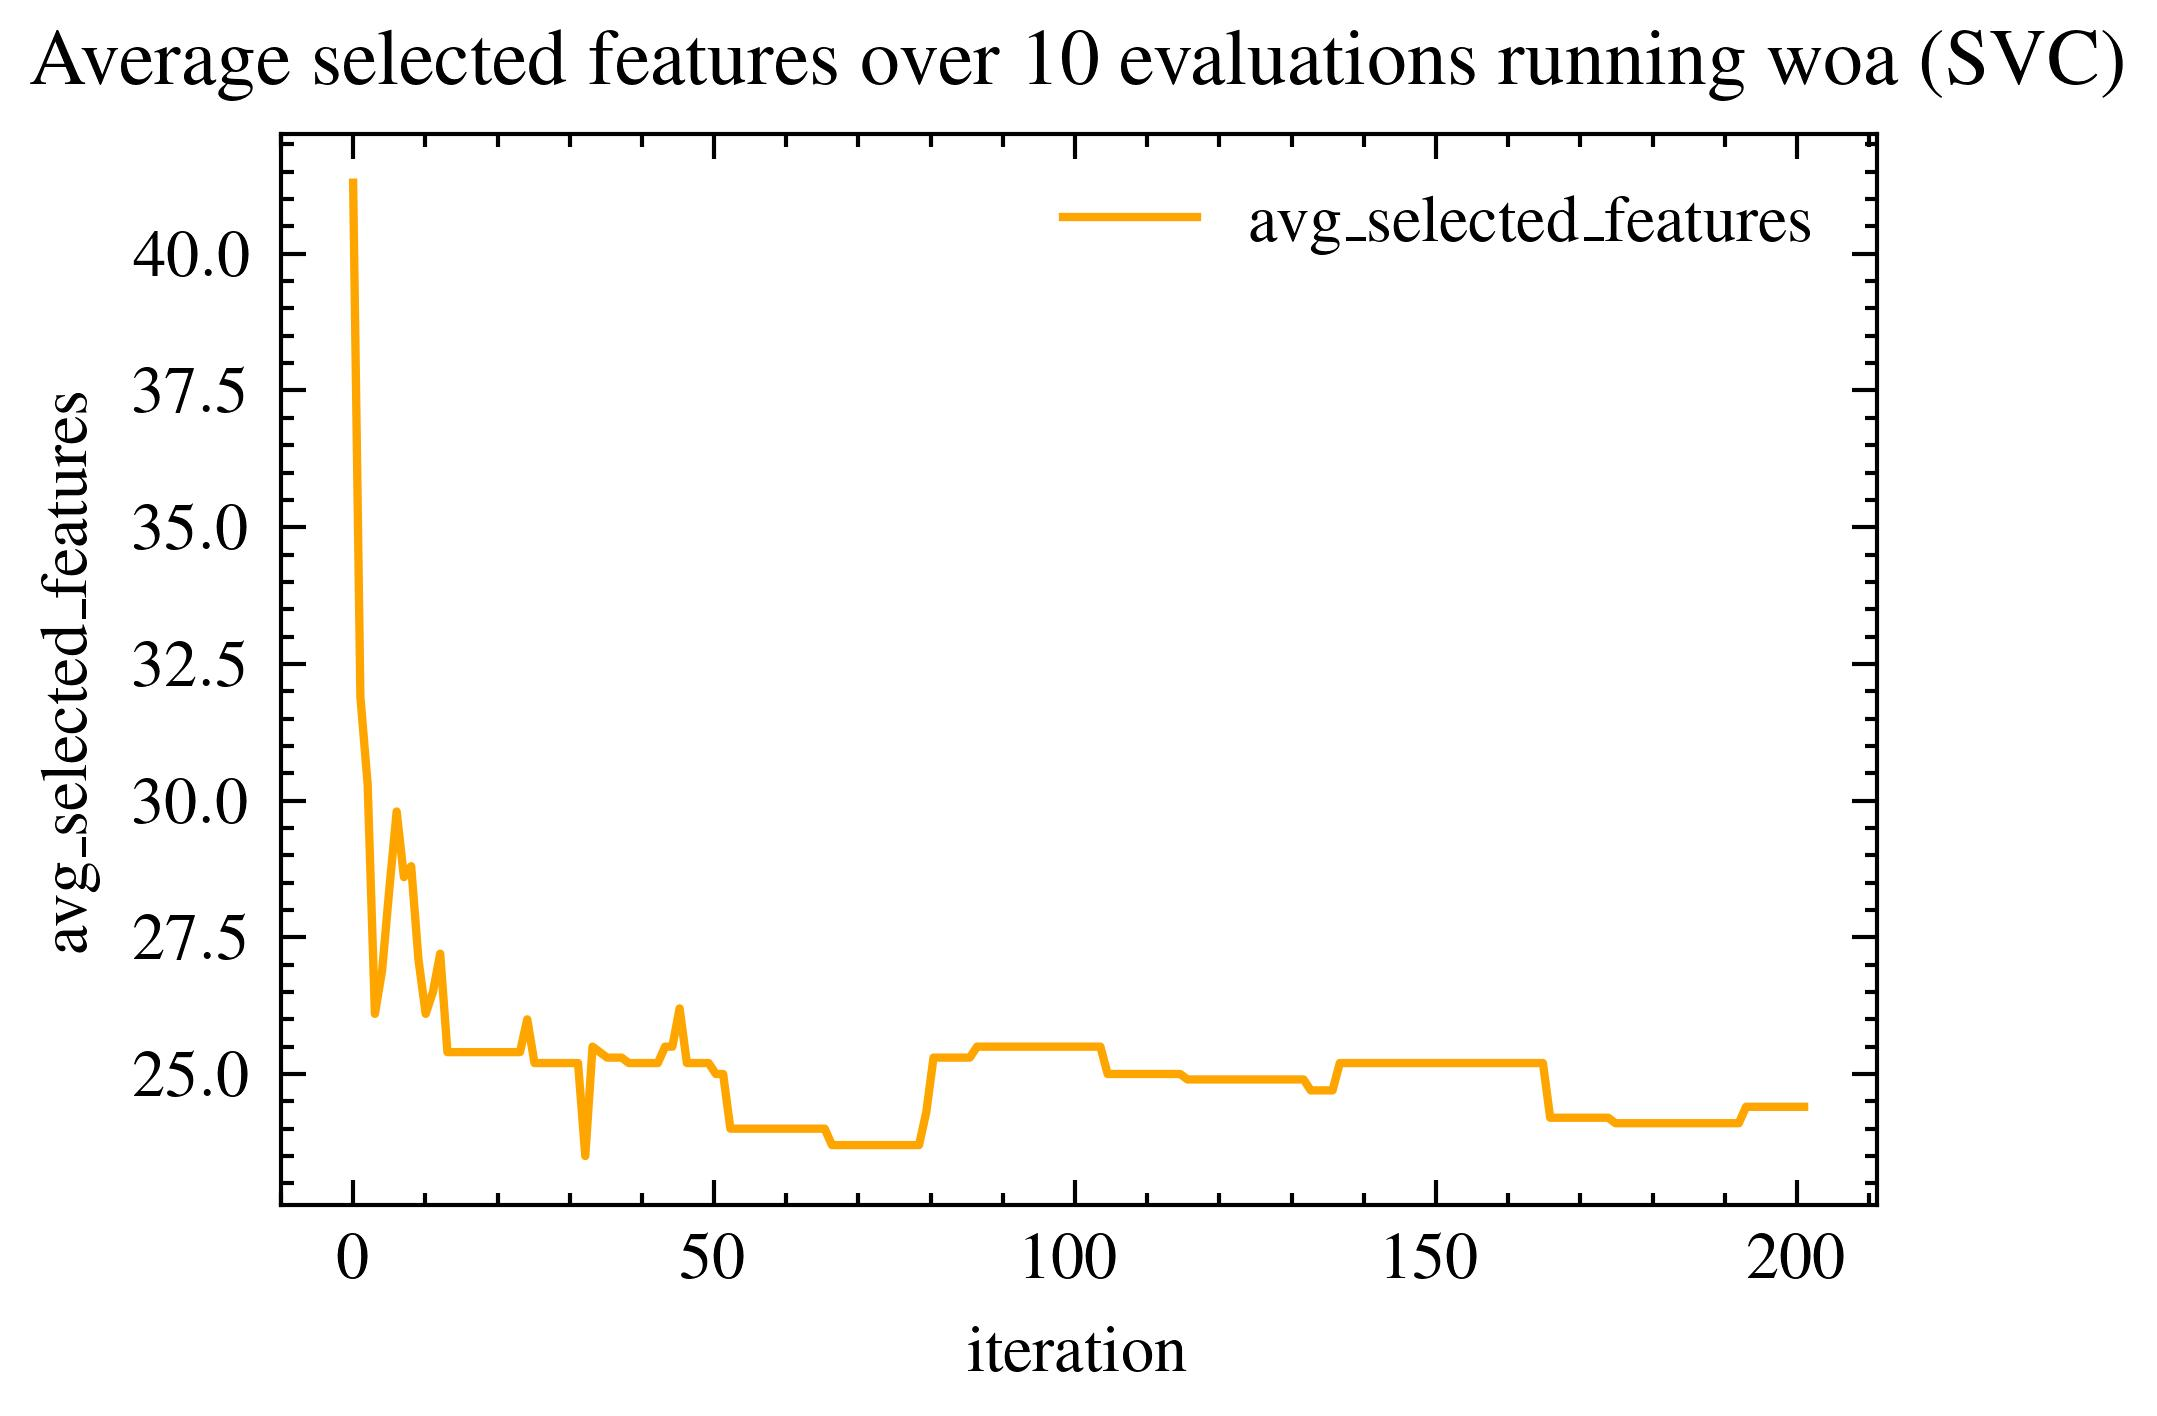
\includegraphics[width=\textwidth]{imagenes/fitness_charts/img/binary/spectf-heart/SVC_n_features_over_10_evaluations_woa_binary_spectf-heart.jpg}
        \caption{spectf-heart}
    \end{subfigure}
    \begin{subfigure}[htp]{0.45\textwidth}
        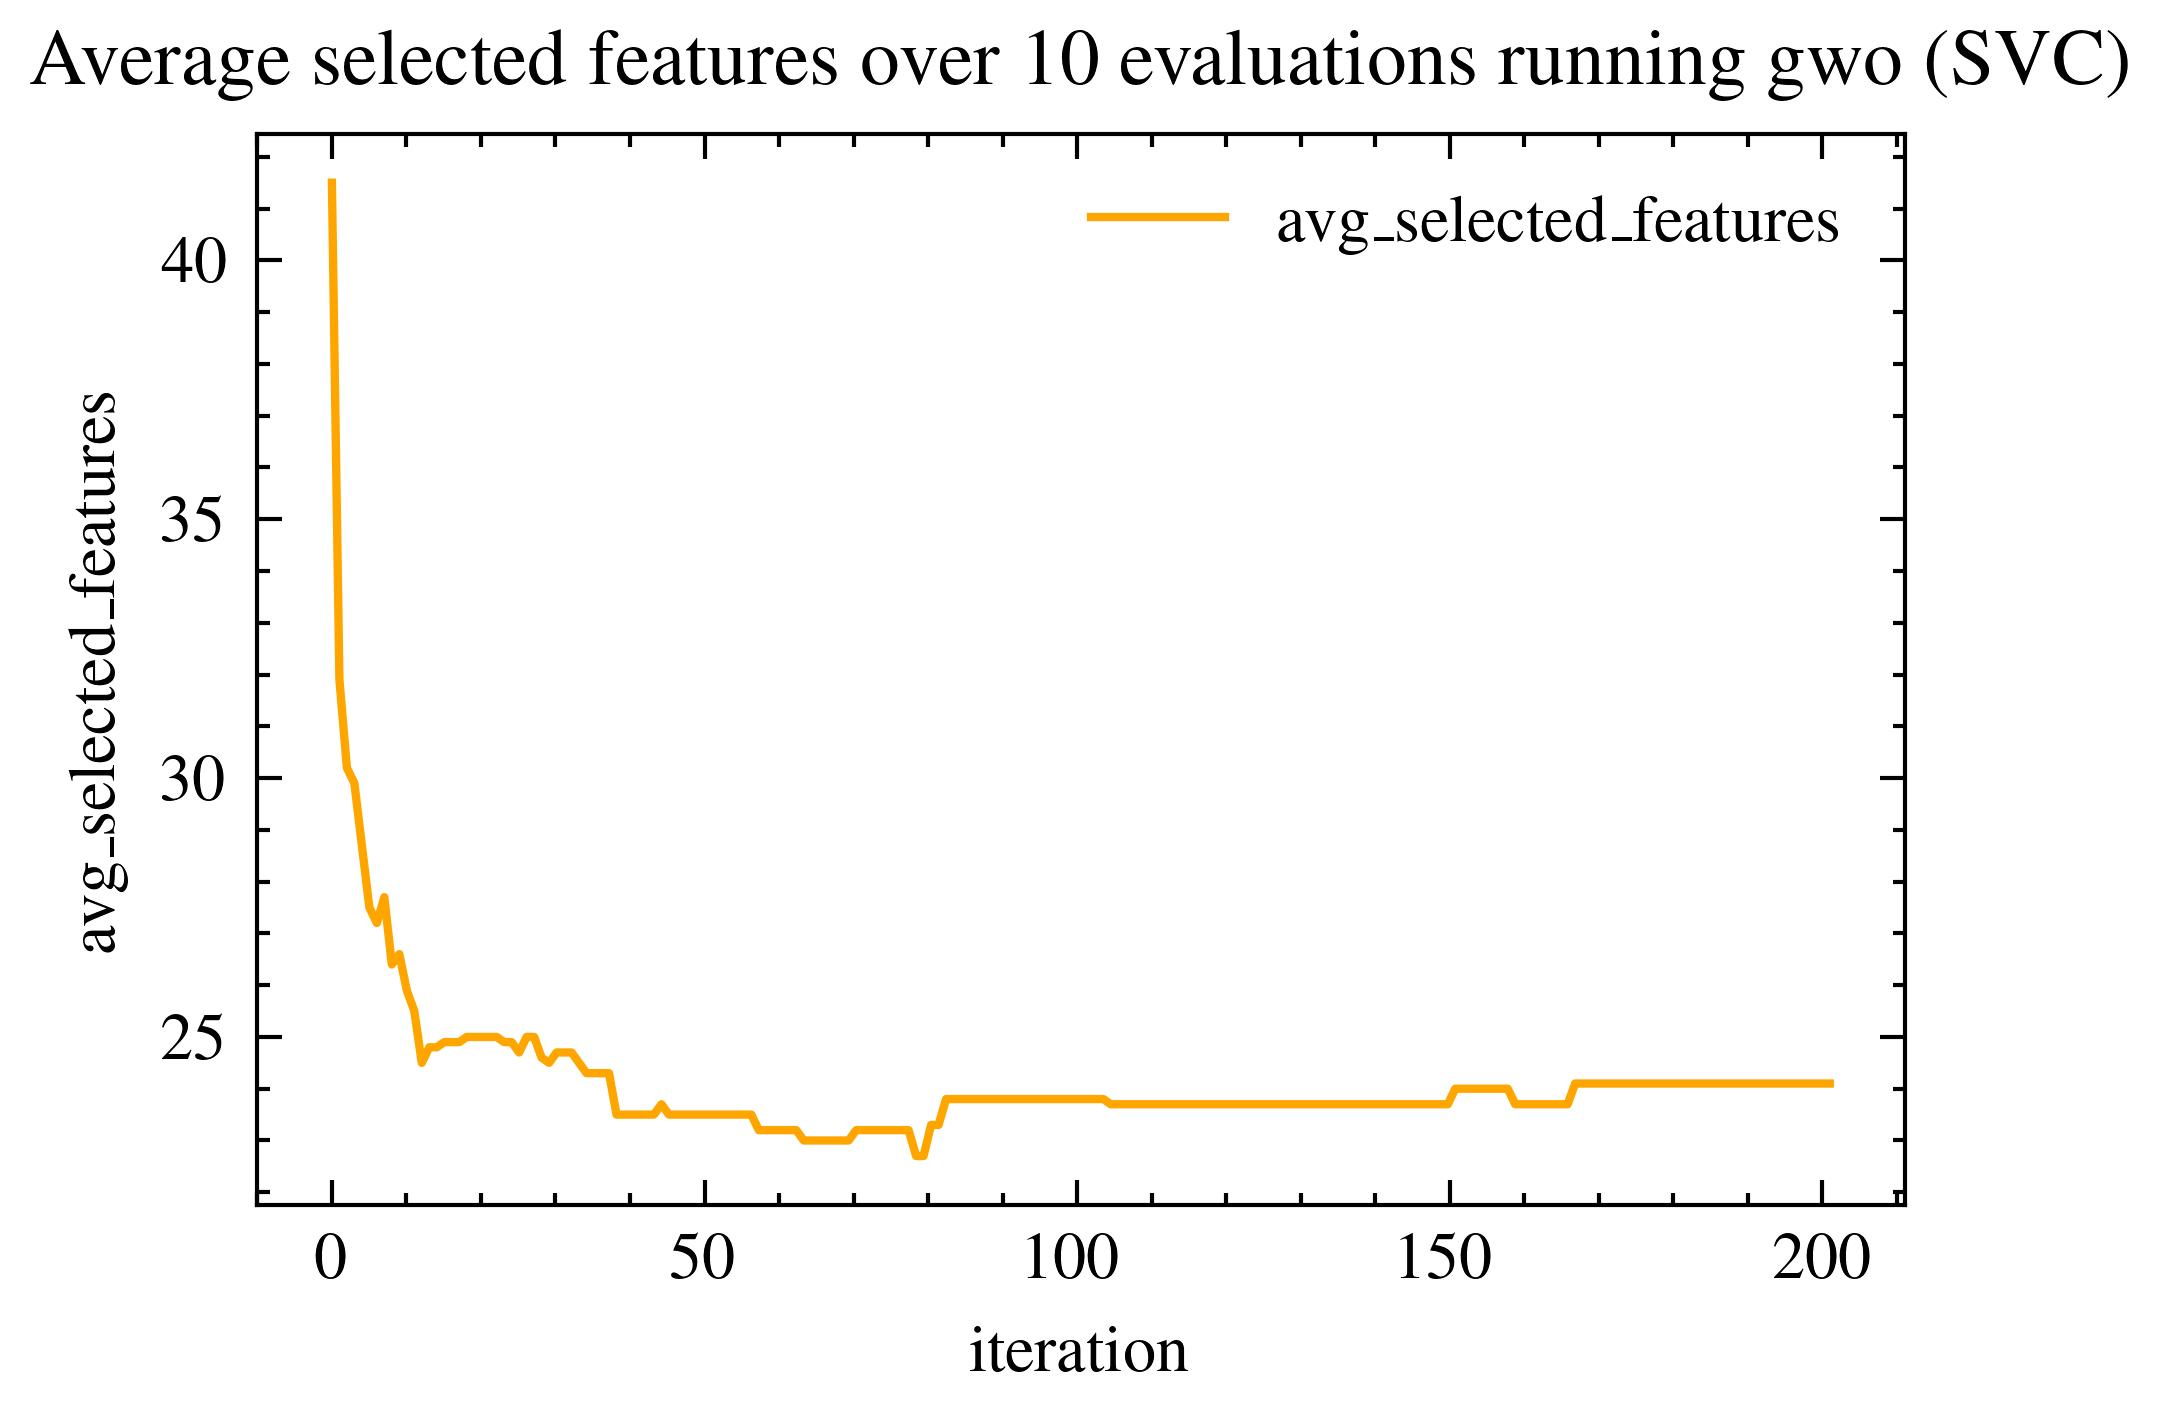
\includegraphics[width=\textwidth]{imagenes/fitness_charts/img/binary/spectf-heart/SVC_n_features_over_10_evaluations_gwo_binary_spectf-heart.jpg}
        \caption{spectf-heart}
    \end{subfigure}

    \begin{subfigure}[htp]{0.45\textwidth}
        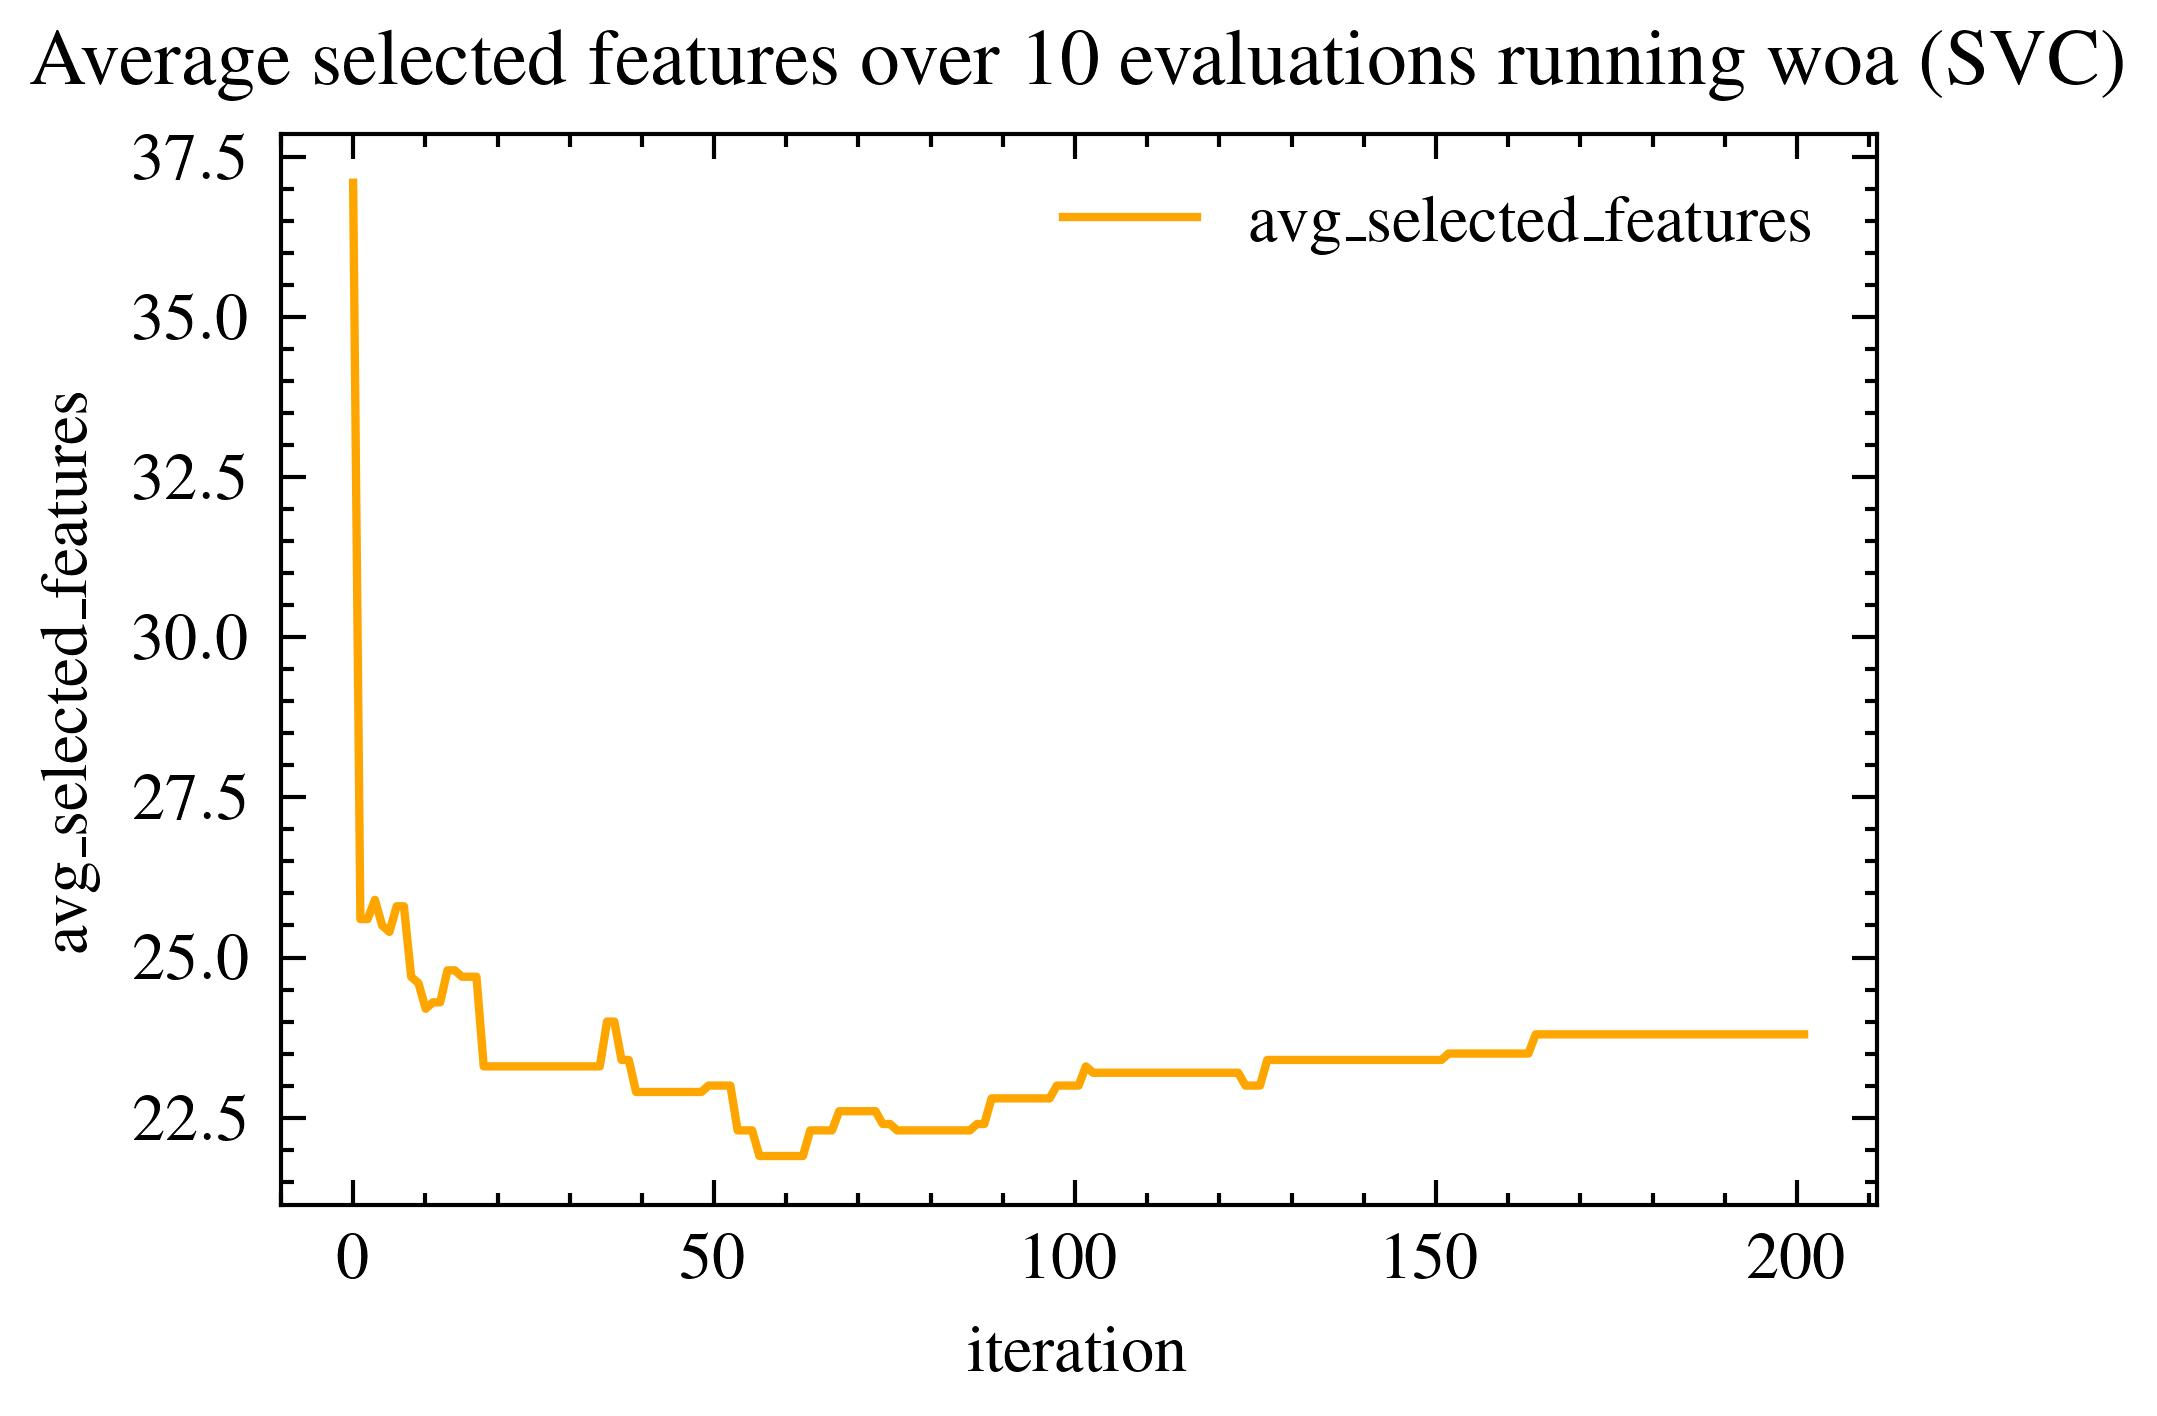
\includegraphics[width=\textwidth]{imagenes/fitness_charts/img/binary/waveform5000/SVC_n_features_over_10_evaluations_woa_binary_waveform5000.jpg}
        \caption{waveform5000}
    \end{subfigure}
    \begin{subfigure}[htp]{0.45\textwidth}
        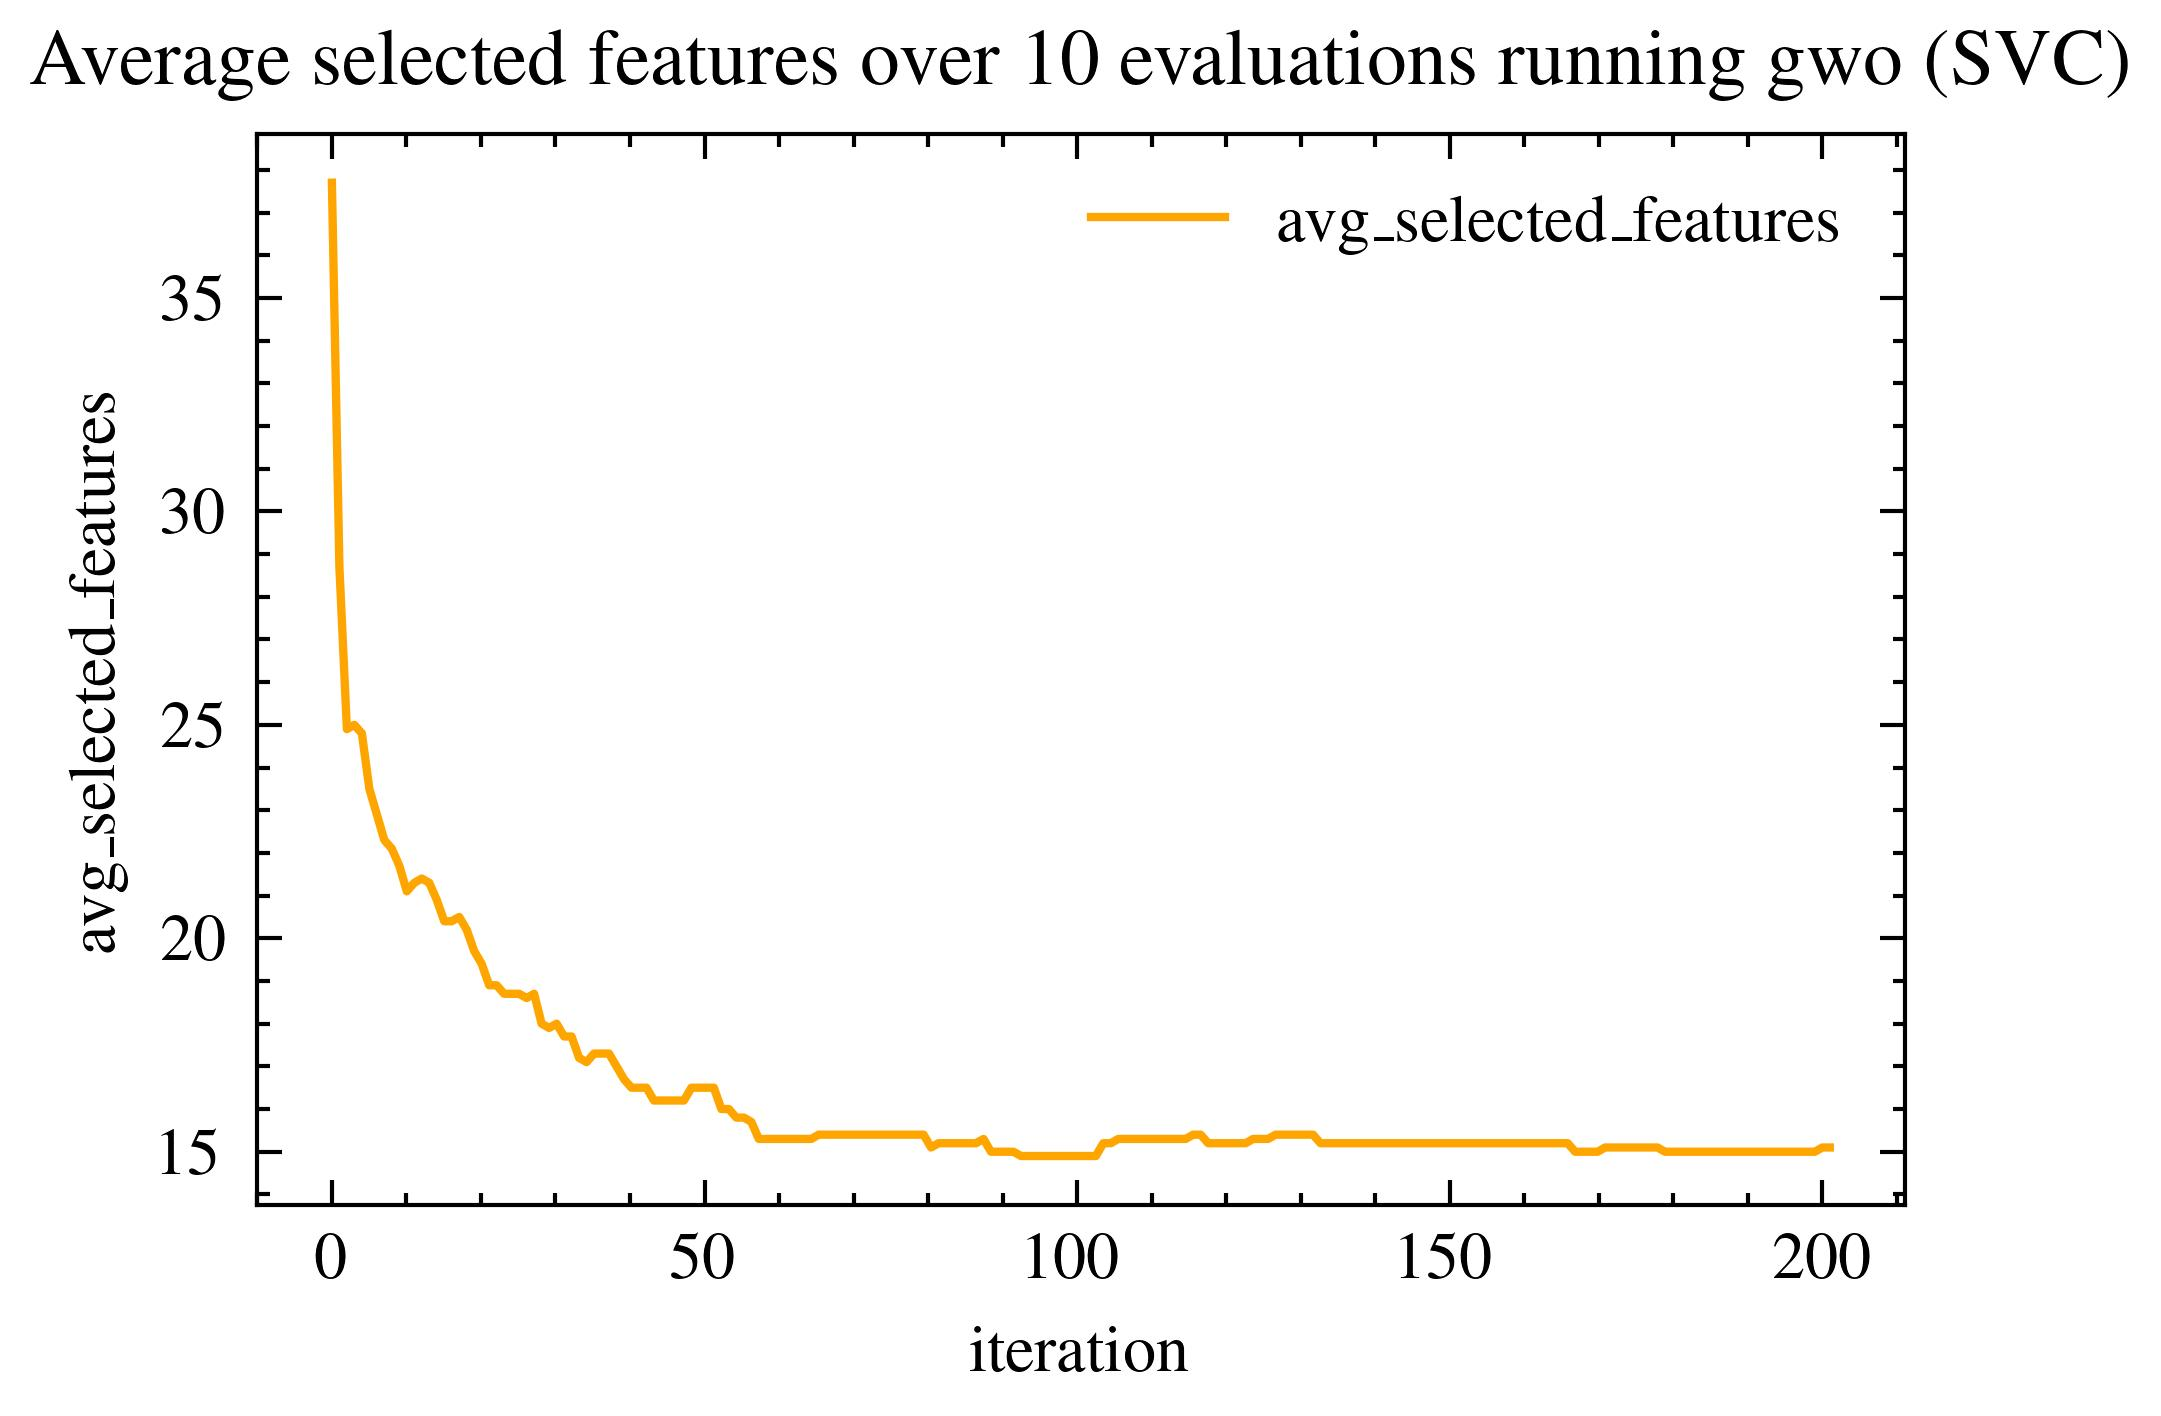
\includegraphics[width=\textwidth]{imagenes/fitness_charts/img/binary/waveform5000/SVC_n_features_over_10_evaluations_gwo_binary_waveform5000.jpg}
        \caption{waveform5000}
    \end{subfigure}

    \begin{subfigure}[htp]{0.45\textwidth}
        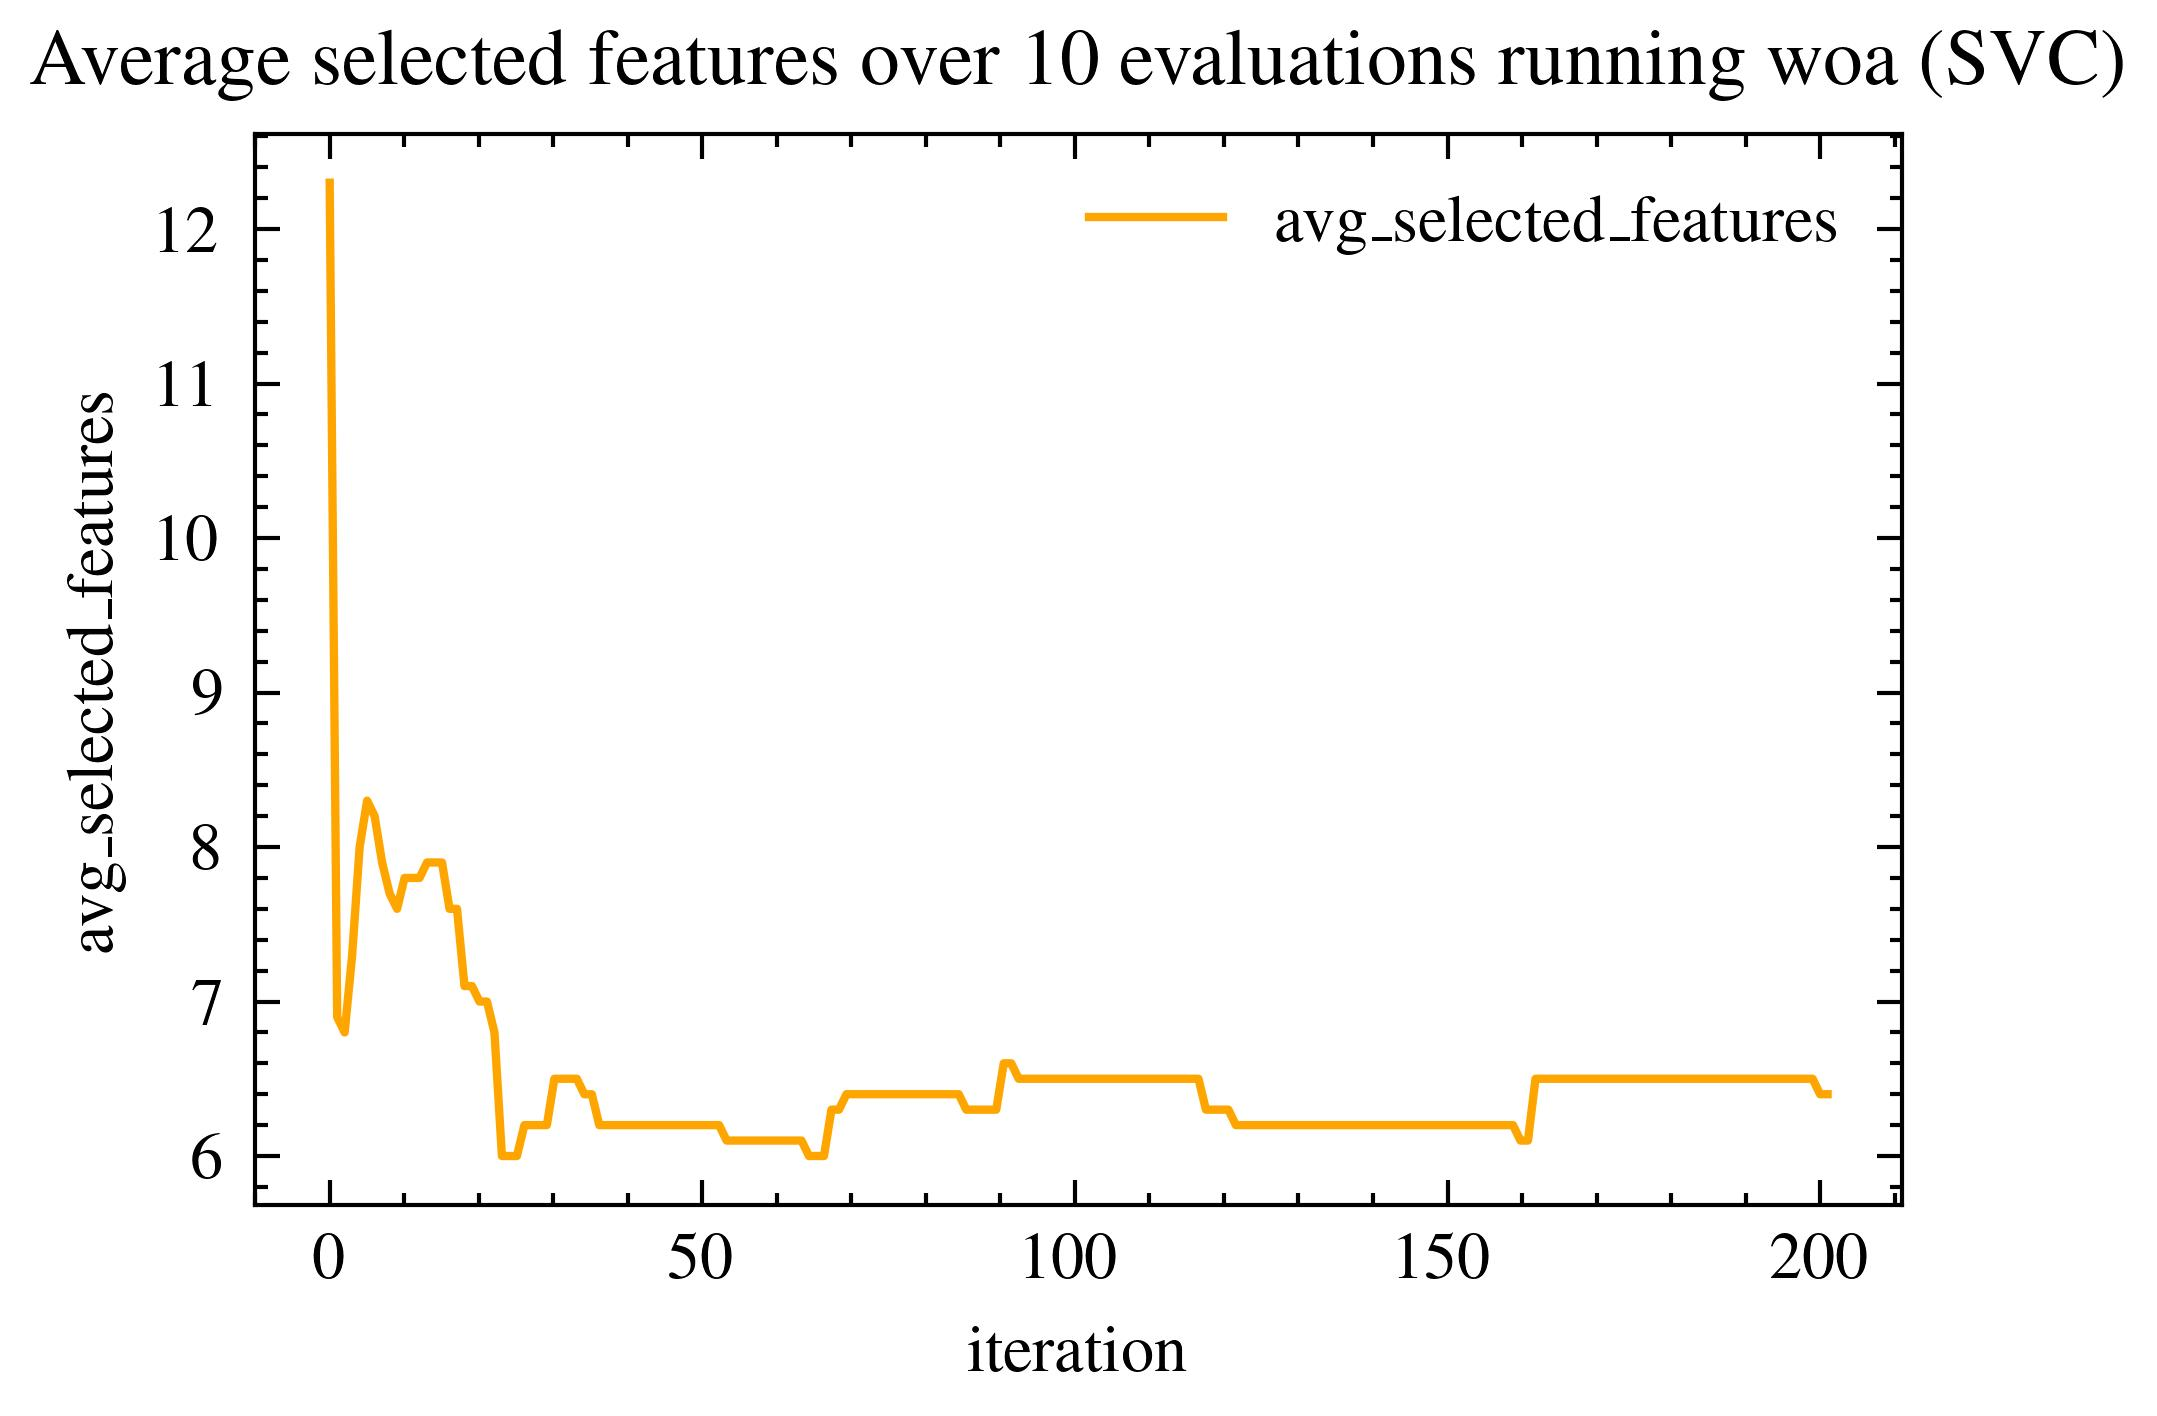
\includegraphics[width=\textwidth]{imagenes/fitness_charts/img/binary/wine/SVC_n_features_over_10_evaluations_woa_binary_wine.jpg}
        \caption{wine}
    \end{subfigure}
    \begin{subfigure}[htp]{0.45\textwidth}
        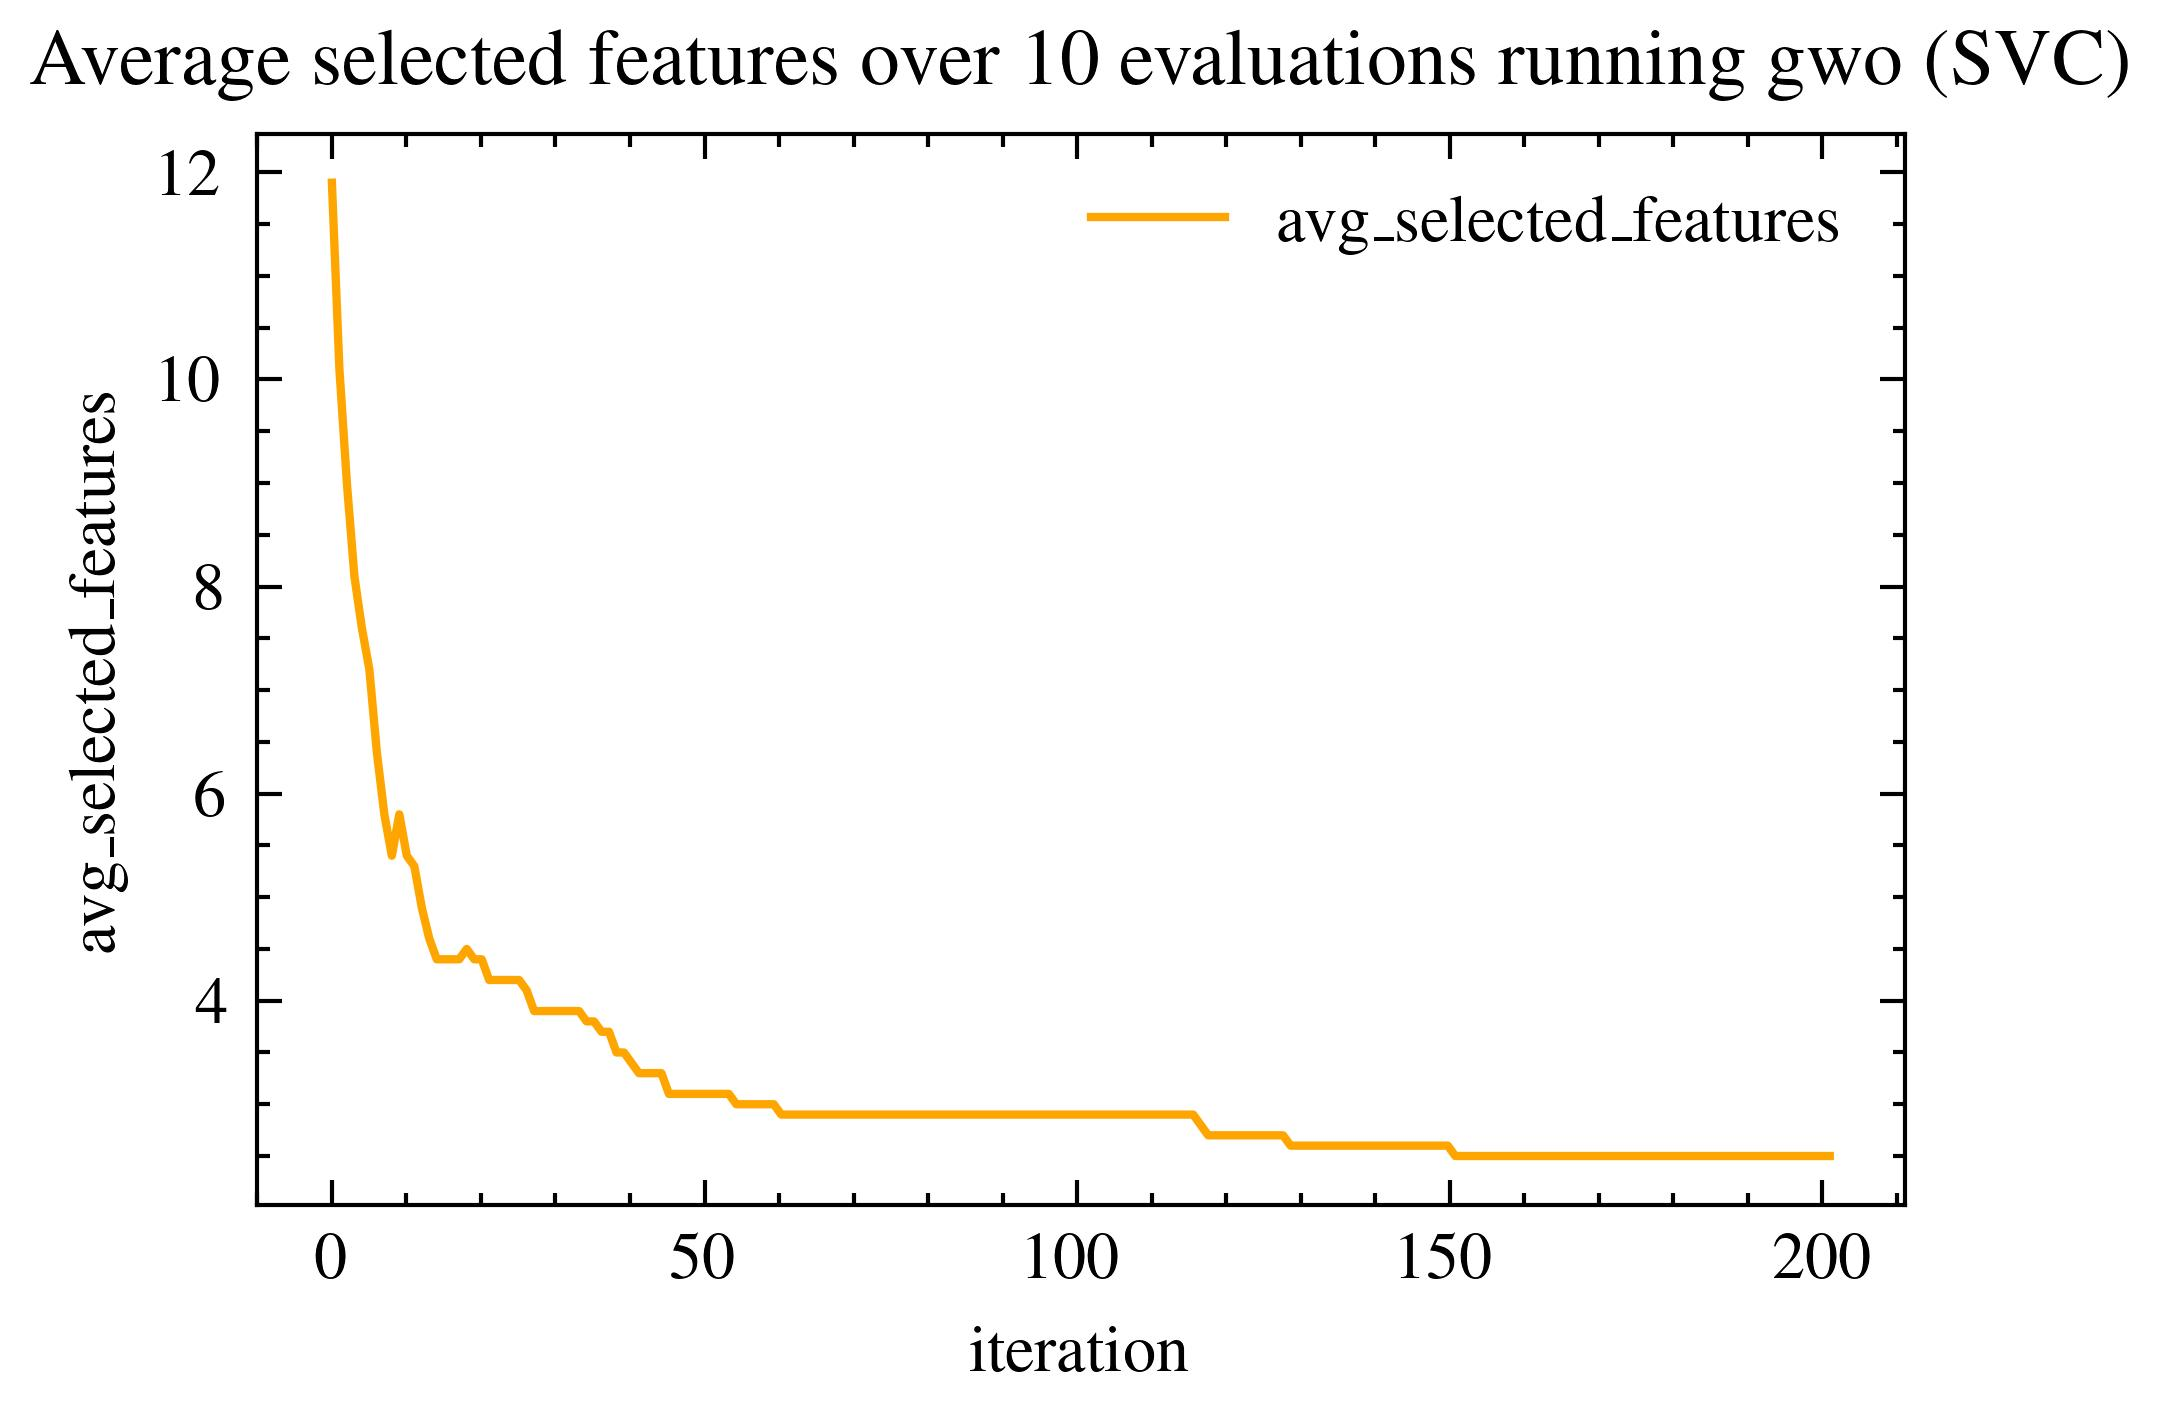
\includegraphics[width=\textwidth]{imagenes/fitness_charts/img/binary/wine/SVC_n_features_over_10_evaluations_gwo_binary_wine.jpg}
        \caption{wine}
    \end{subfigure}
    \caption{Reducción de características en bWOA y bGWO}
    \label{fig:svc_selected_rate_gwo_woa_bin}
\end{figure}

Es en cambio en la comparación en la métrica de reducción de características se aprecia que \textbf{bGWO} presenta una diferencia notable con respecto a \textbf{bWOA}. Puede observarse gráficamente en las figuras \ref{fig:svc_selected_rate_gwo_woa_bin} como \textbf{bWOA} reduce considerablemente menos que \textbf{bGWO}. Comprobarse también que las diferencias entre ambos son estadísticamente significativas \ref{tab:pval_corr_gwo_woa-bin_knn}, \ref{tab:pval_corr_gwo_woa-bin_svc}

\begin{table}[htp]
    \centering
    \begin{tabular}{lll}
        \toprule
        {}  & gwo                & woa                \\
        \midrule
        gwo & -                  & - (\textbf{0.001}) \\
        woa & + (\textbf{0.001}) & -                  \\
        \bottomrule
    \end{tabular}
    \caption{P-valores tras corrección entre bGWO y bWOA - knn}
    \label{tab:pval_corr_gwo_woa-bin_knn}
\end{table}

\begin{table}[htp]
    \centering
    \begin{tabular}{lll}
        \toprule
        {}  & gwo                & woa                \\
        \midrule
        gwo & -                  & - (\textbf{0.002}) \\
        woa & + (\textbf{0.002}) & -                  \\
        \bottomrule
    \end{tabular}
    \caption{P-valores tras corrección entre bGWO y bWOA - svc}
    \label{tab:pval_corr_gwo_woa-bin_svc}
\end{table}

Por tanto, pese a no haber una diferencia estadística suficientemente fuerte entre los resultados de precisión de ambos algoritmos, si la hay en la reducción de características. Por ello se puede afirmar que \textbf{bGWO} es más interesante que \textbf{bWOA}.

\clearpage
\subsection{Tiempo de ejecución}
Una última métrica muy importante a analizar es el tiempo de ejecución. Por definición, la mayoría de metaheurísticas deberían ser rápidas, al menos en comparación a algoritmos exactos, pues es en sustitución de estos donde brillan realmente. En el caso concreto del problema de selección de características es algo a tener muy en cuenta, pues unos de los cuellos de botella principales en el entrenamiento de grandes modelos es el tiempo de ejecución. Por tanto, en esta sección se procederá a analizar varios algoritmos y sus diferencias en cuanto a tiempos.\\[6pt]

Los resultados arrojan dos algoritmos con diferencias relevantes, \textbf{bFA} con una diferencia positiva y \textbf{bABCO} con una diferencia negativa. Véase en la table \ref{tab:mean_time_knn_bin}. El resto de algoritmo obtienen tiempos muy similares en todos los conjuntos de datos.

\subsection{Convergencia}
En esta última sub-sección se analizará la convergencia de los diferentes algoritmos. Inicialmente, si se observan las gráficas de convergencia de cada \textit{dataset} \ref{fig:convergencia_svc_1}, \ref{fig:convergencia_svc_2}, \ref{fig:convergencia_knn_1}, \ref{fig:convergencia_knn_2} y se analizan las curvas, se puede decir que absolutamente todos los algoritmos convergen, ya sea a una solución mejor o peor, pero todos lo hacen (incluso \textbf{Dummy}). No hay ninguno en ningún problema que retroceda en cuanto a su valor \textit{fitness} y todos poseen una curva descendiente bastante suave. Con el tiempo, esta curva tiende a alcanzar un límite inferior, como si de una función logarítmica se tratase. Esto indica, que el algoritmo está mejorando cada vez menos porque ha encontrado un óptimo local.

\begin{figure}[htp]
    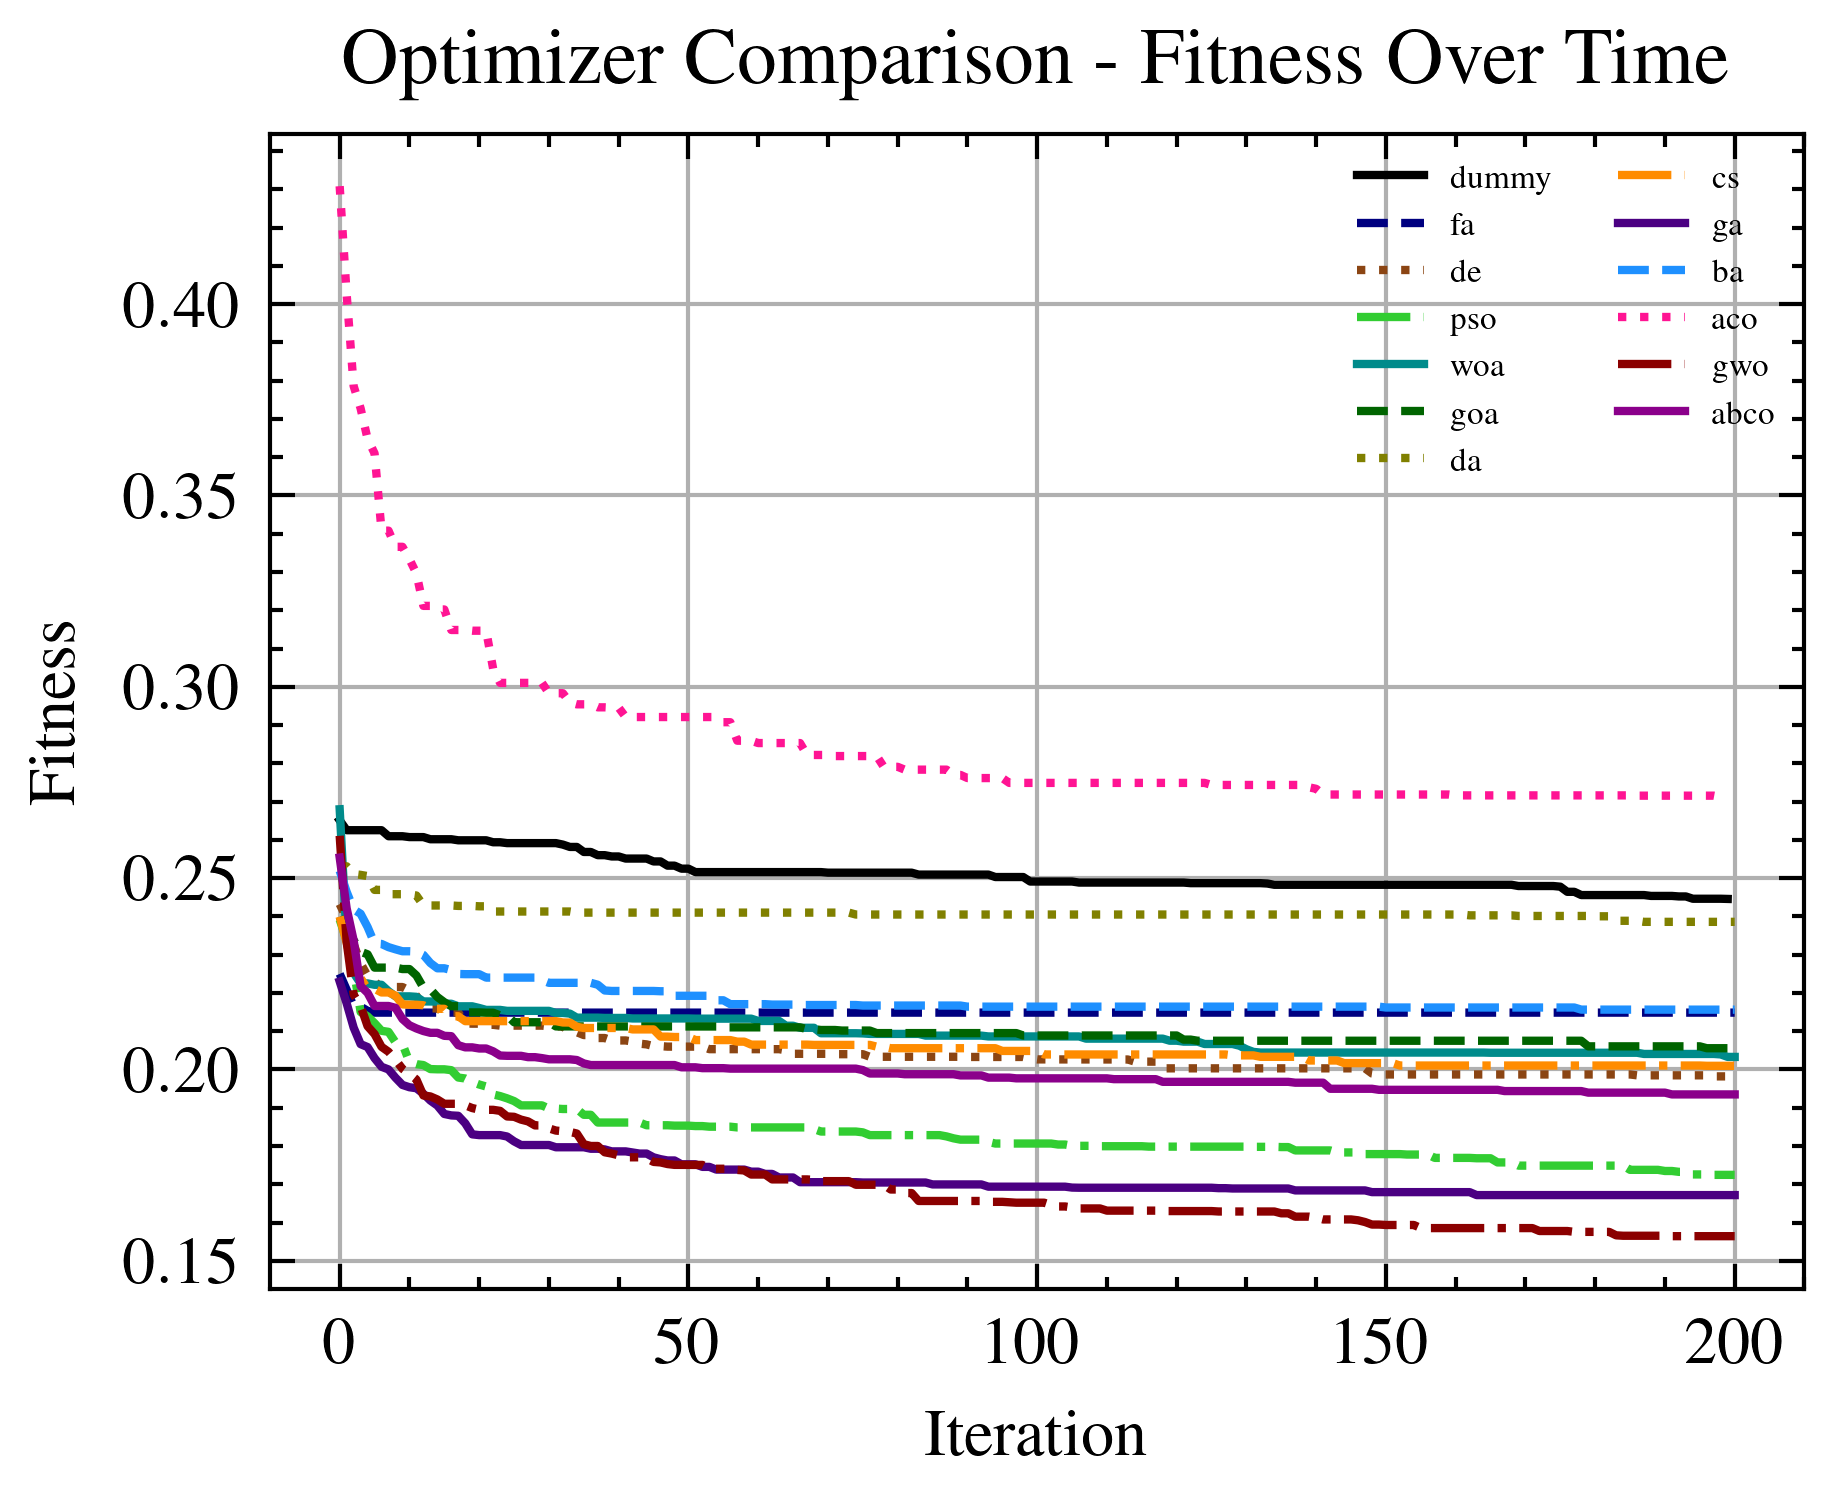
\includegraphics[width=0.8\textwidth]{imagenes/fitness_charts/img/binary/waveform5000/optimizers_fitness_knn.png}
    \caption{Convergencia de todas las metaheurísticas en waveform5000 - knn - binario}
\end{figure}

\begin{figure}[htp]
    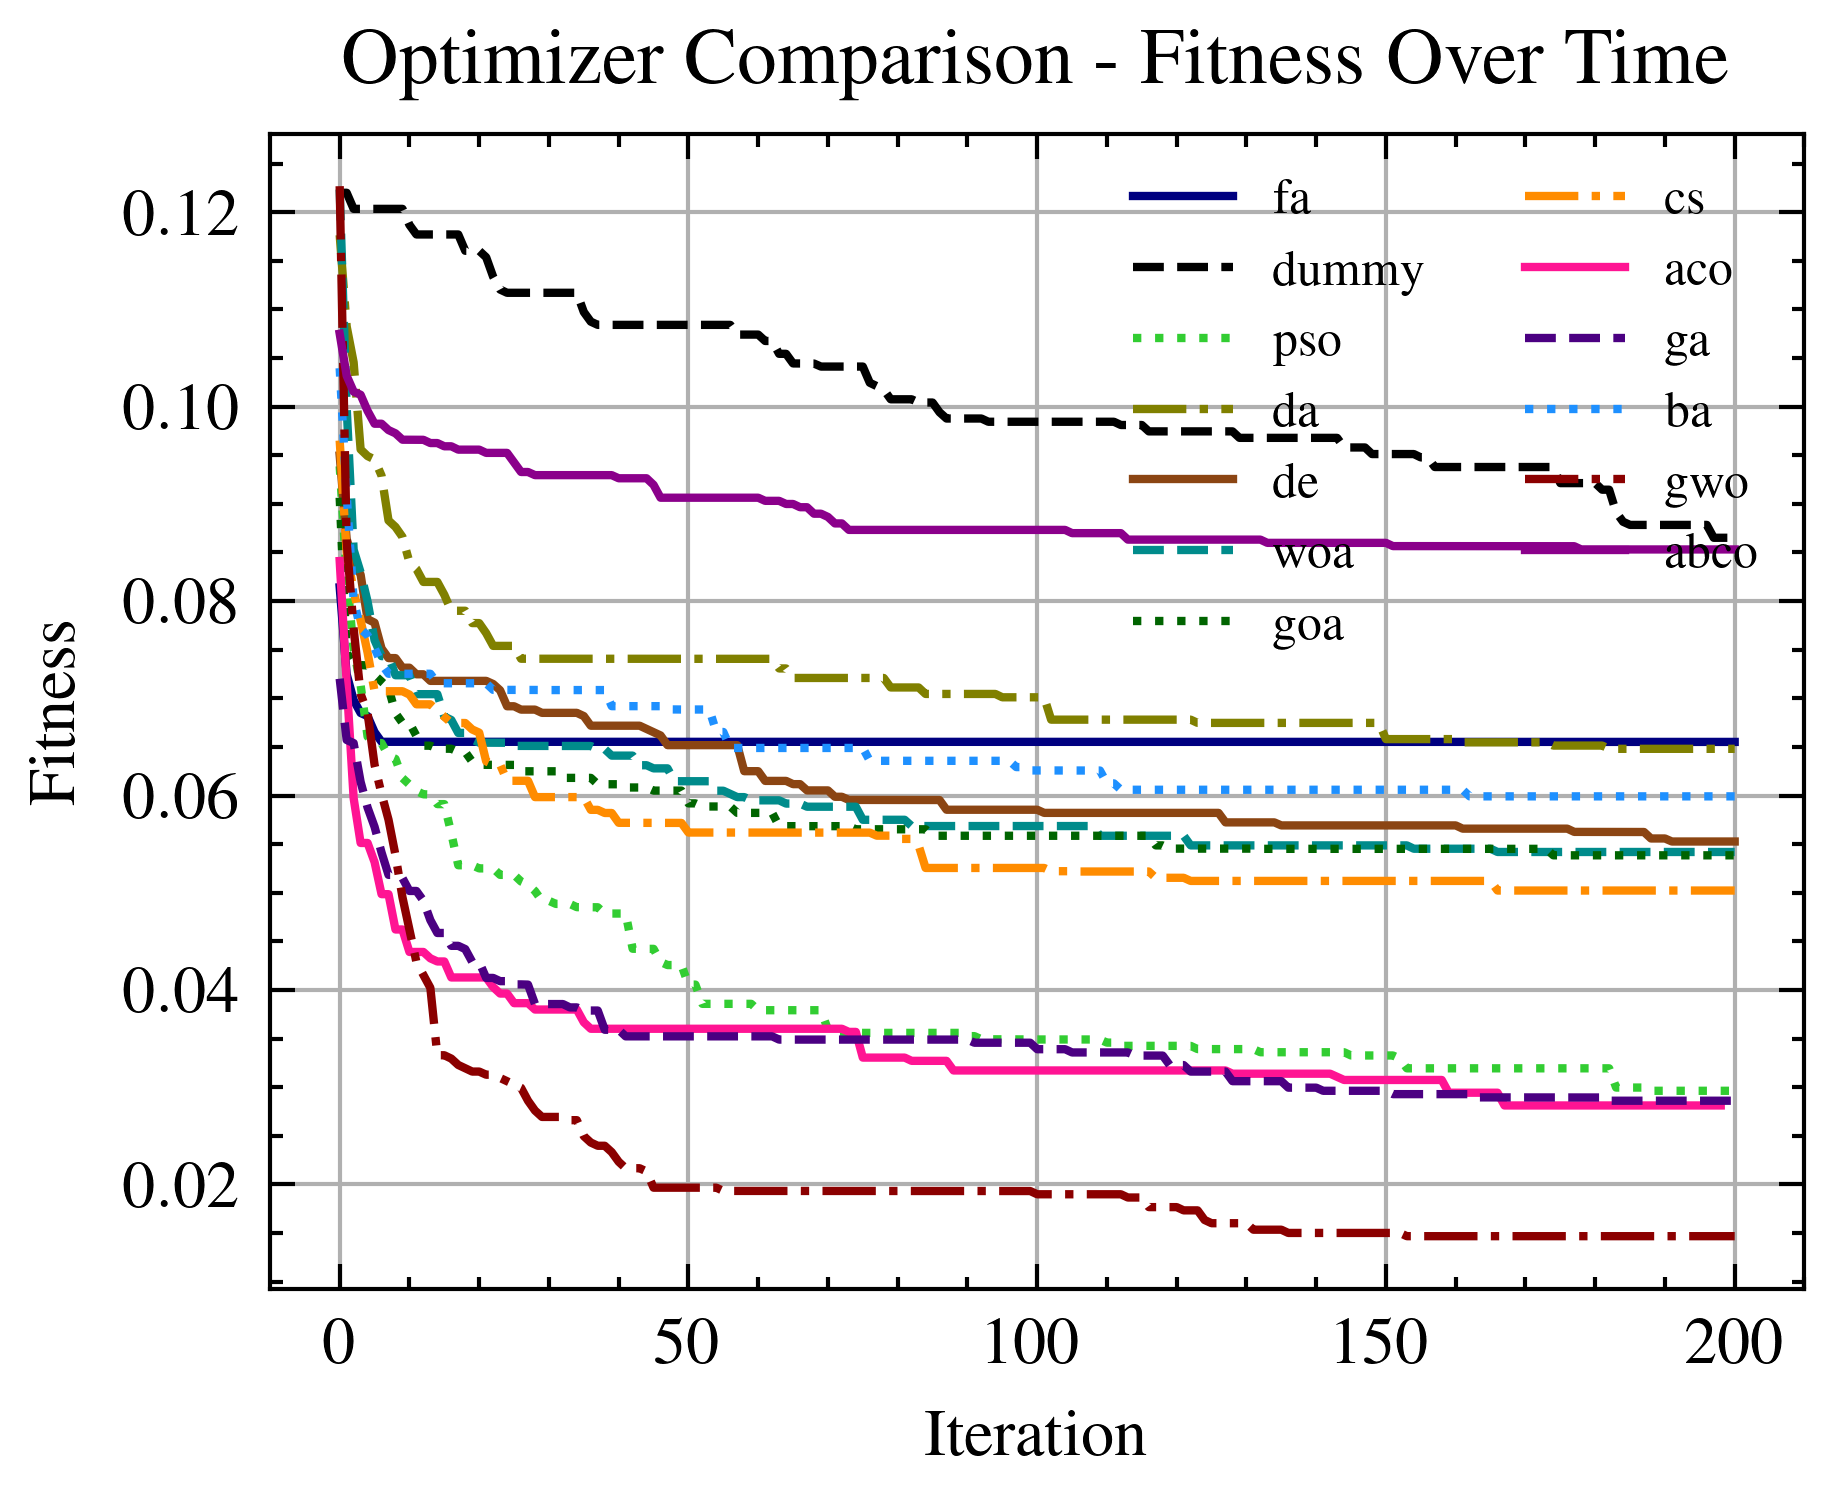
\includegraphics[width=0.8\textwidth]{imagenes/fitness_charts/img/binary/wdbc/optimizers_fitness_knn.png}
    \caption{Convergencia de todas las metaheurísticas en wdbc - knn - binario}
\end{figure}

Claramente, el peor algoritmo y al que más le cuesta converger es \textbf{ACO}. Pese a ello, \textbf{ACO} parece variar mucho en su proceso optimizatorio entre distintos conjuntos de datos.\\[6pt]
Otro algoritmo que converge más lentamente que el resto es el \textbf{bDA} y el \textbf{bGOA}. Por ejemplo, en el problema de \textit{diabetes}, representado en la figura~\ref{fig:convergencia_diabetes_svc}, se puede apreciar que el \textbf{bDA} es mejor que \textbf{bGOA} y que ambos son los más lentos a excepción del \textbf{bDummy}. \\[6pt]

Pese a las dificultades de algunos algoritmos, todos convergen correctamente en todos los conjuntos de datos, lo cual es esperable.

\section{Continuo}
En esta sección se analizarán las metaheurísticas en su versión real o continua. En este apartado se ha optado por no usar en las comparativas el algoritmo \textbf{ACO} en su versión continua. Dado que \textbf{ACO} fue concebido como un algoritmo binario y que sus implementaciones, pese a haberlas, se alejan bastante de la idea original y distorsionan el algoritmo, se ha tomado la decisión de no incluirlo. Por tanto, se compararan las versiones continuas, que son las originales de cada algoritmo, entre sí. En el caso de \textbf{GA} se hace uso de operadores especiales, según se explicó en anteriores capítulos, para adaptarlo a un contexto de codificación real, siendo el único que requería de una modificación de los operadores.\\[6pt]
La estrategia seguida en los algoritmos continuos es distinta a los binarios. En los binarios, como se ha mencionado, se eligen características, mientras que otras son rechazadas. Por otro lado, en los continuos no se llegan a descartar características, sino que se ponderan por importancia. Desde este punto de vista, se podría pensar que los continuos tienen mayor maniobrabilidad en el entrenamiento, pues se encargan de ajustar pesos en vez de eliminarlos, por tanto trabajan con más información y más rango de acción. A priori, mayor cantidad de información es mejor. El análisis realizado en esta sección tratará de comprobar como se comportan los continuos para el problema de selección de características, partiendo del hecho de que ninguno de ellos ha sido diseñado específicamente para ello, como sí es el caso de los binarios.

\subsection{General}
De igual forma que en el apartado anterior sobre los binarios, se procede a presentar una serie de resultados iniciales en forma de rankings, los cuales permitirán una visión general del comportamiento.

\begin{figure}[htp]
    \centering
    \begin{subfigure}[htp]{1\textwidth}
        \includegraphics[width=\textwidth]{imagenes/fitness_charts/img/real/rankings_knn_avg.png}
        \caption{Ranking por fitness para knn - real}
        \label{fig:ranking_knn_real}
    \end{subfigure}
    \begin{subfigure}[htp]{1\textwidth}
        \includegraphics[width=\textwidth]{imagenes/fitness_charts/img/real/rankings_svc_avg.png}
        \caption{Ranking por fitness para svc - real}
        \label{fig:ranking_svc_real}
    \end{subfigure}
    \caption{Rankings para fitness - real}
\end{figure}

Según se observa en las figuras de \ref{fig:ranking_knn_real} y \ref{fig:ranking_svc_real}, lo que más llama la atención es que hay algoritmos clasificados peor incluso que el \textbf{Dummy}, el cual es totalmente aleatorio. Estos son \textbf{DA} en \textbf{SVC} y \textbf{GOA} en ambos clasificadores. Parecen obtener resultados pésimos, pese a ser sus versiones originales.\\[6pt]
En cambio, algoritmos que ya habían destacado en binario, lo vuelven a hacer en continuo, además con una puntuación muy buena con respecto al resto de metaheurísticas. Estos son \textbf{CS} y \textbf{GWO}. En el top de mejores optimizadores entran además los algoritmos de \textbf{BA} y \textbf{WOA}, los cuales si bien no eran malos en binario, no eran los mejores, más bien promedio. Se mantiene el algoritmo genético dentro del top de los cinco mejores. Los algoritmos clásicos ocupan el grueso del medio en los rankings.

\subsection{Variabilidad}

\begin{figure}[htp]
    \centering
    \begin{subfigure}[htp]{0.5\textwidth}
        \centering
        \includegraphics[width=\textwidth]{imagenes/fitness_charts/results/real/waveform5000/optimizer_boxplot_fitness_knn_r.png}
        \caption{waveform5000}
        \label{fig:boxplot_waveform5000_real}
    \end{subfigure}
    \begin{subfigure}[htp]{0.5\textwidth}
        \centering
        \includegraphics[width=\textwidth]{imagenes/fitness_charts/results/real/yeast/optimizer_boxplot_fitness_knn_r.png}
        \caption{yeast}
        \label{fig:boxplot_yeast_real}
    \end{subfigure}
    \begin{subfigure}[htp]{0.5\textwidth}
        \centering
        \includegraphics[width=\textwidth]{imagenes/fitness_charts/results/real/spectf-heart/optimizer_boxplot_fitness_knn_r.png}
        \caption{spectf-heart}
        \label{fig:boxplot_spectf-heart_real}
    \end{subfigure}
    \begin{subfigure}[htp]{0.5\textwidth}
        \centering
        \includegraphics[width=\textwidth]{imagenes/fitness_charts/results/real/dermatology/optimizer_boxplot_fitness_knn_r.png}
        \caption{dermatology}
        \label{fig:boxplot_dermatology_real}
    \end{subfigure}
    \caption{\textit{Boxplots} para knn - real}
    \label{fig:combined_boxplots}
\end{figure}

En las figuras presentadas en \ref{fig:boxplot_waveform5000_real}, \ref{fig:boxplot_yeast_real}, \ref{fig:boxplot_spectf-heart_real}, \ref{fig:boxplot_dermatology_real} pueden observarse los resultados obtenidos para los conjuntos de datos \textbf{waveform5000}, \textbf{yeast}, \textbf{spectf-heart} y \textbf{dermatology} usando el clasificador \textbf{kNN}.\\[6pt]

A primera vista, destaca ver la \textit{desviación típica} de los resultados de la mayoría de propuestas, pues es bastante pequeña en general. Esto da a entender que los resultados obtenidos en las $10$ pruebas difieren poco entre sí y por tanto estos son bastante robustos. \\[6pt]
Destacar como algoritmos muy notorios el \textbf{CS}, \textbf{GWO}, \textbf{BA} y \textbf{PSO}, que parecen obtener muy buenos resultados y ser bastante compactos en cuanto a su desviación. Por el contrario, algoritmos como \textbf{GOA} parecen obtener un rendimiento más bajo y ser muy variables en comparación al resto. Si se observan las colas de \textbf{GOA} en las figuras, esta es más larga por arriba, hacia valores muy altos de \textit{fitness} (se está minimizando, por tanto no es bueno). No representa el grueso de los resultados, pues es la cola, que representa un $25\%$ de los datos, pero sigue siendo un valor más que importante.\\[6pt]

\subsection{Fitness}
En la comparación de \textit{fitness}, los mejores algoritmos, según se ha podido observar anteriormente, eran \textbf{CS} y \textbf{GWO}. Los peores algoritmos son \textbf{GOA} y \textbf{DA}. Es interesante ver como estos dos últimos han bajado tanto de puesto en comparación a su versión en binario, teniendo en cuenta que originalmente estas dos metaheurísticas son continuas. También es muy destacable ver como los mejores lo son por mucho y los peores también, es decir, hay una diferencia bastante grande de calidad entre buenos y peores, mientras que en binario los saltos en rankings no eran tan grandes.

\subsubsection{Mejor vs Resto}
Se procede a comparar al mejor algoritmo en continuo con el resto de metaheurísticas. Este es el \textbf{CS}, el cual puede verse como supera al resto en los rankings \ref{fig:ranking_knn_real} y \ref{fig:ranking_svc_real}. Haciendo los procesados estadísticos pertinentes, se obtiene los siguientes resultados expuestos en las tablas \ref{tab:tab:p_values_fitness_real_knn} y \ref{tab:tab:p_values_fitness_real_svc}.\\[6pt]
Pese a no haberse realizado aún la corrección post hoc de \textit{Holms}, se pueden observar resultados concluyentes para algoritmos como \textbf{GOA}. Claramente, incluso tras corrección, los resultados de \textbf{CS} son superiores frente a este y con una seguridad más que suficiente para afirmar que \textbf{CS} es mejor que \textbf{GOA}. Ocurre lo mismo con \textbf{DA} y otros tantos. En las tablas con los p-valores post hoc, se pueden apreciar los resultados estadísticos finales para \textbf{kNN} \ref{tab:p-values_cs_rest_real_knn} y \textbf{SVC} \ref{tab:p-values_cs_rest_real_svc}.

\begin{table}
    \centering
    \begin{tabular}{lllll}
        \toprule
        {}    & Original  & Holm           & Hommel         & Hochberg       \\
        \midrule
        fa    & 6.104E-05 & \textbf{0.001} & \textbf{0.001} & \textbf{0.001} \\
        goa   & 6.104E-05 & \textbf{0.001} & \textbf{0.001} & \textbf{0.001} \\
        dummy & 1.221E-04 & \textbf{0.001} & \textbf{0.001} & \textbf{0.001} \\
        abco  & 3.052E-04 & \textbf{0.002} & \textbf{0.002} & \textbf{0.002} \\
        da    & 0.001     & \textbf{0.008} & \textbf{0.008} & \textbf{0.008} \\
        de    & 0.003     & \textbf{0.016} & \textbf{0.016} & \textbf{0.016} \\
        ga    & 0.010     & 0.050          & 0.050          & 0.050          \\
        pso   & 0.035     & 0.141          & 0.106          & 0.134          \\
        ba    & 0.045     & 0.141          & 0.134          & 0.134          \\
        woa   & 0.222     & 0.444          & 0.444          & 0.444          \\
        gwo   & 0.934     & 0.934          & 0.934          & 0.934          \\
        \bottomrule
    \end{tabular}
    \caption{P-valores de CS vs el resto - knn - real}
    \label{tab:p-values_cs_rest_real_knn}
\end{table}

\begin{table}
    \centering
    \begin{tabular}{lllll}
        \toprule
        {}    & Original  & Holm           & Hommel         & Hochberg       \\
        \midrule
        da    & 6.104E-05 & \textbf{0.001} & \textbf{0.001} & \textbf{0.001} \\
        goa   & 1.221E-04 & \textbf{0.001} & \textbf{0.001} & \textbf{0.001} \\
        de    & 3.052E-04 & \textbf{0.003} & \textbf{0.003} & \textbf{0.003} \\
        dummy & 0.002     & \textbf{0.016} & \textbf{0.016} & \textbf{0.016} \\
        fa    & 0.005     & \textbf{0.034} & \textbf{0.034} & \textbf{0.034} \\
        pso   & 0.018     & 0.110          & 0.092          & 0.110          \\
        abco  & 0.028     & 0.140          & 0.112          & 0.140          \\
        ba    & 0.045     & 0.178          & 0.178          & 0.178          \\
        ga    & 0.151     & 0.454          & 0.454          & 0.454          \\
        woa   & 0.320     & 0.640          & 0.561          & 0.561          \\
        gwo   & 0.561     & 0.640          & 0.561          & 0.561          \\
        \bottomrule
    \end{tabular}
    \caption{P-valores de CS vs el resto - svc - real}
    \label{tab:p-values_cs_rest_real_svc}
\end{table}

Se pueden observar en las tablas que \textbf{CS} obtiene resultados significativos para \textbf{DA}, \textbf{GOA}, \textbf{DE} y \textbf{FA}. El algoritmo \textbf{ABCO} solo obtiene resultados significativamente peores con el uso de \textbf{kNN}.\\[6pt]
Con ello, se puede afirmar que \textbf{CS} es un algoritmo muy interesante para los problemas de clasificación en continuo, superando a al resto con resultados muy superiores.

\subsubsection{Clásicos vs Modernos}
Agrupando algoritmos usando las tablas de rankings \ref{tab:ranking_fitness_real_svc}, \ref{tab:ranking_fitness_real_knn} se pueden hacer tres grupos, tanto por la diferencias de ponderación como por antigüedad de algoritmos (clásicos vs modernos). Por lo general, los clásicos, a excepción del \textbf{GA} en \textbf{SVC}, obtienen resultados muy buenos, pero promedios. Los modernos, sin embargo, se dividen en dos grupos, entre los peores y los mejores.\\[6pt]
Esto indica que algunos de los algoritmos modernos son capaces de superar a los clásicos en sus versiones originales, como \textbf{WOA} o \textbf{BA}, los cuales obtuvieron resultados promedios en las comparaciones binarias.\\[6pt]
Pese a ello, los clásicos obtienen resultados igualmente buenos en sus versiones originales. \textbf{PSO} y \textbf{GA} posicionan alto y superando a gran cantidad de modernos. Se mantienen muy bien con el paso de los años y su sencillez algorítmica sigue demostrando que la filosofía de \textit{la navaja de Ockham} sigue estando muy presente.\\[6pt]
Y aunque sigan existiendo algoritmos confiables y robustos como algunos de los clásicos, con el tiempo se van diseñando algunos como \textbf{GWO} o \textbf{CS} capaces de mejorar los resultados.

\subsubsection{GA vs DE}
Los algoritmos \textbf{DE} y \textbf{GA} comparten varios conceptos y similitudes fundamentales. Emplean operadores de variación, como la mutación y la recombinación (\textit{crossover}), para introducir diversidad en la población y generar nuevas soluciones. Ambos algoritmos seleccionan soluciones de la población actual (padres) para generar nuevas soluciones (descendientes) mediante estos operadores de variación. Posteriormente, las nuevas soluciones reemplazan a las soluciones menos aptas en la población, siguiendo una estrategia de selección basada en la función de \textit{fitness}.\\[6pt]
\textbf{DE} de hecho, como se ha explicado en secciones anteriores, surgió como una alternativa más refinada a \textbf{GA} para codificaciones continuas. Tiene sentido por tanto comparar ambas metaheurísticas entre sí.\\[6pt]
Comparando sus resultados en los rankings \ref{fig:ranking_knn_real} y \ref{fig:ranking_svc_real}, parece que \textbf{GA} es superior a \textbf{DE}, lo cual es interesante, pues \textbf{DE} fué, como ya se ha explicado, diseñado específicamente para continuos, mientras que los genéticos para los binarios.\\[6pt]
Si bien es cierto, los algoritmos genéticos han recibido más atención por parte del público general y quizá hayan sido más desarrollados durante el tiempo, explorando nuevos tipos de operadores. Además los genéticos han sido usado en multitud de problemas continuos con éxito. Comparando ambos, se obtienen los siguientes p-valores en \ref{tab:pval_corr_ga_de-real_knn} y \ref{tab:pval_corr_ga_de-real_svc}.

\begin{table}[htp]
    \centering
    \begin{tabular}{lll}
        \toprule
        {} & de        & ga        \\
        \midrule
        de & -         & + (0.188) \\
        ga & - (0.188) & -         \\
        \bottomrule
    \end{tabular}
    \caption{P-valores tras corrección entre GA y DE - knn - real}
    \label{tab:pval_corr_ga_de-real_knn}
\end{table}

\begin{table}[htp]
    \centering
    \begin{tabular}{lll}
        \toprule
        {} & de                 & ga                 \\
        \midrule
        de & -                  & + (\textbf{0.041}) \\
        ga & - (\textbf{0.041}) & -                  \\
        \bottomrule
    \end{tabular}
    \caption{P-valores tras corrección entre GA y DE - svc - real}
    \label{tab:pval_corr_ga_de-real_svc}
\end{table}

En la versión de \textbf{SVC} se obtiene resultados estadísticamente significativos a favor de la superioridad de la versión continua de \textbf{GA} contra el algoritmo \textbf{DE}.

\subsection{Clasificación y reducción}

\begin{figure}[htp]
    \centering
    \begin{subfigure}[htp]{1\textwidth}
        \includegraphics[width=\textwidth]{imagenes/fitness_charts/img/real/rankings_knn_selected_rate.png}
        \caption{Ranking por selección de características para knn - real}
        \label{fig:ranking_knn_real_sel_rate}
    \end{subfigure}
    \begin{subfigure}[htp]{1\textwidth}
        \includegraphics[width=\textwidth]{imagenes/fitness_charts/img/real/rankings_svc_selected_rate.png}
        \caption{Ranking por selección de características para svc - real}
        \label{fig:ranking_svc_real_sel_rate}
    \end{subfigure}
    \caption{Rankings para selección de características - real}
\end{figure}

Dada la naturaleza de la composición de la ecuación de \textit{fitness}, cabría esperar resultados prácticamente iguales en \textit{accuracy}. Este hecho fue comprobado con los algoritmos binarios en secciones anteriores. Pese a ello, al observar los rankings (\ref{tab:ranking_accuracy_real_sv}, \ref{tab:ranking_accuracy_real_kn}) se percibe una diferencia con respecto al \textit{fitness}. El mejor es \textbf{GWO}, y no por mucho. De hecho, todos obtienen ponderaciones similares, por lo que parece que todos son capaces de obtener valores de precisión muy buenos. Por ello se procede a realizar un análisis con el foco de la reducción de dimensiones, que podría ser la métrica discriminatoria entre algoritmos.\\[6pt]
Las figuras \ref{fig:ranking_svc_real_sel_rate} y \ref{fig:ranking_knn_real_sel_rate} muestran los rankings de las mejores opciones en cuanto a reducción de atributos. Da la casualidad, que los resultados son iguales que en los rankings de \textit{fitness} en \ref{tab:ranking_fitness_real_svc} y \ref{tab:ranking_fitness_real_knn}. La única diferencia notable es que la discriminación entre posiciones crece incluso más si cabe que midiendo el \textit{fitness}. Los mejores son muy buenos y los peores pésimos en reducción.\\[6pt]
De hecho, si se observan las tablas de p-valores en \textit{accuracy} en \ref{tab:p-values_accuracy_real_svc} y \ref{tab:p-values_accuracy_real_knn}, se aprecia que en los resultados, apenas hay diferencias si quiera cercanas a la significatividad estadística, la cual se ha limitado por debajo del $5\%$. Por ello, cabría esperar esta desigualdad y diferencias tan grandes en reducción de características. Todos parecen obtener una precisión más o menos buena, pero solo algunos reducen (y lo hacen mucho).

\subsubsection{Mejor vs Peor}
\begin{figure}[htp]
    \centering
    \begin{subfigure}[htp]{0.45\textwidth}
        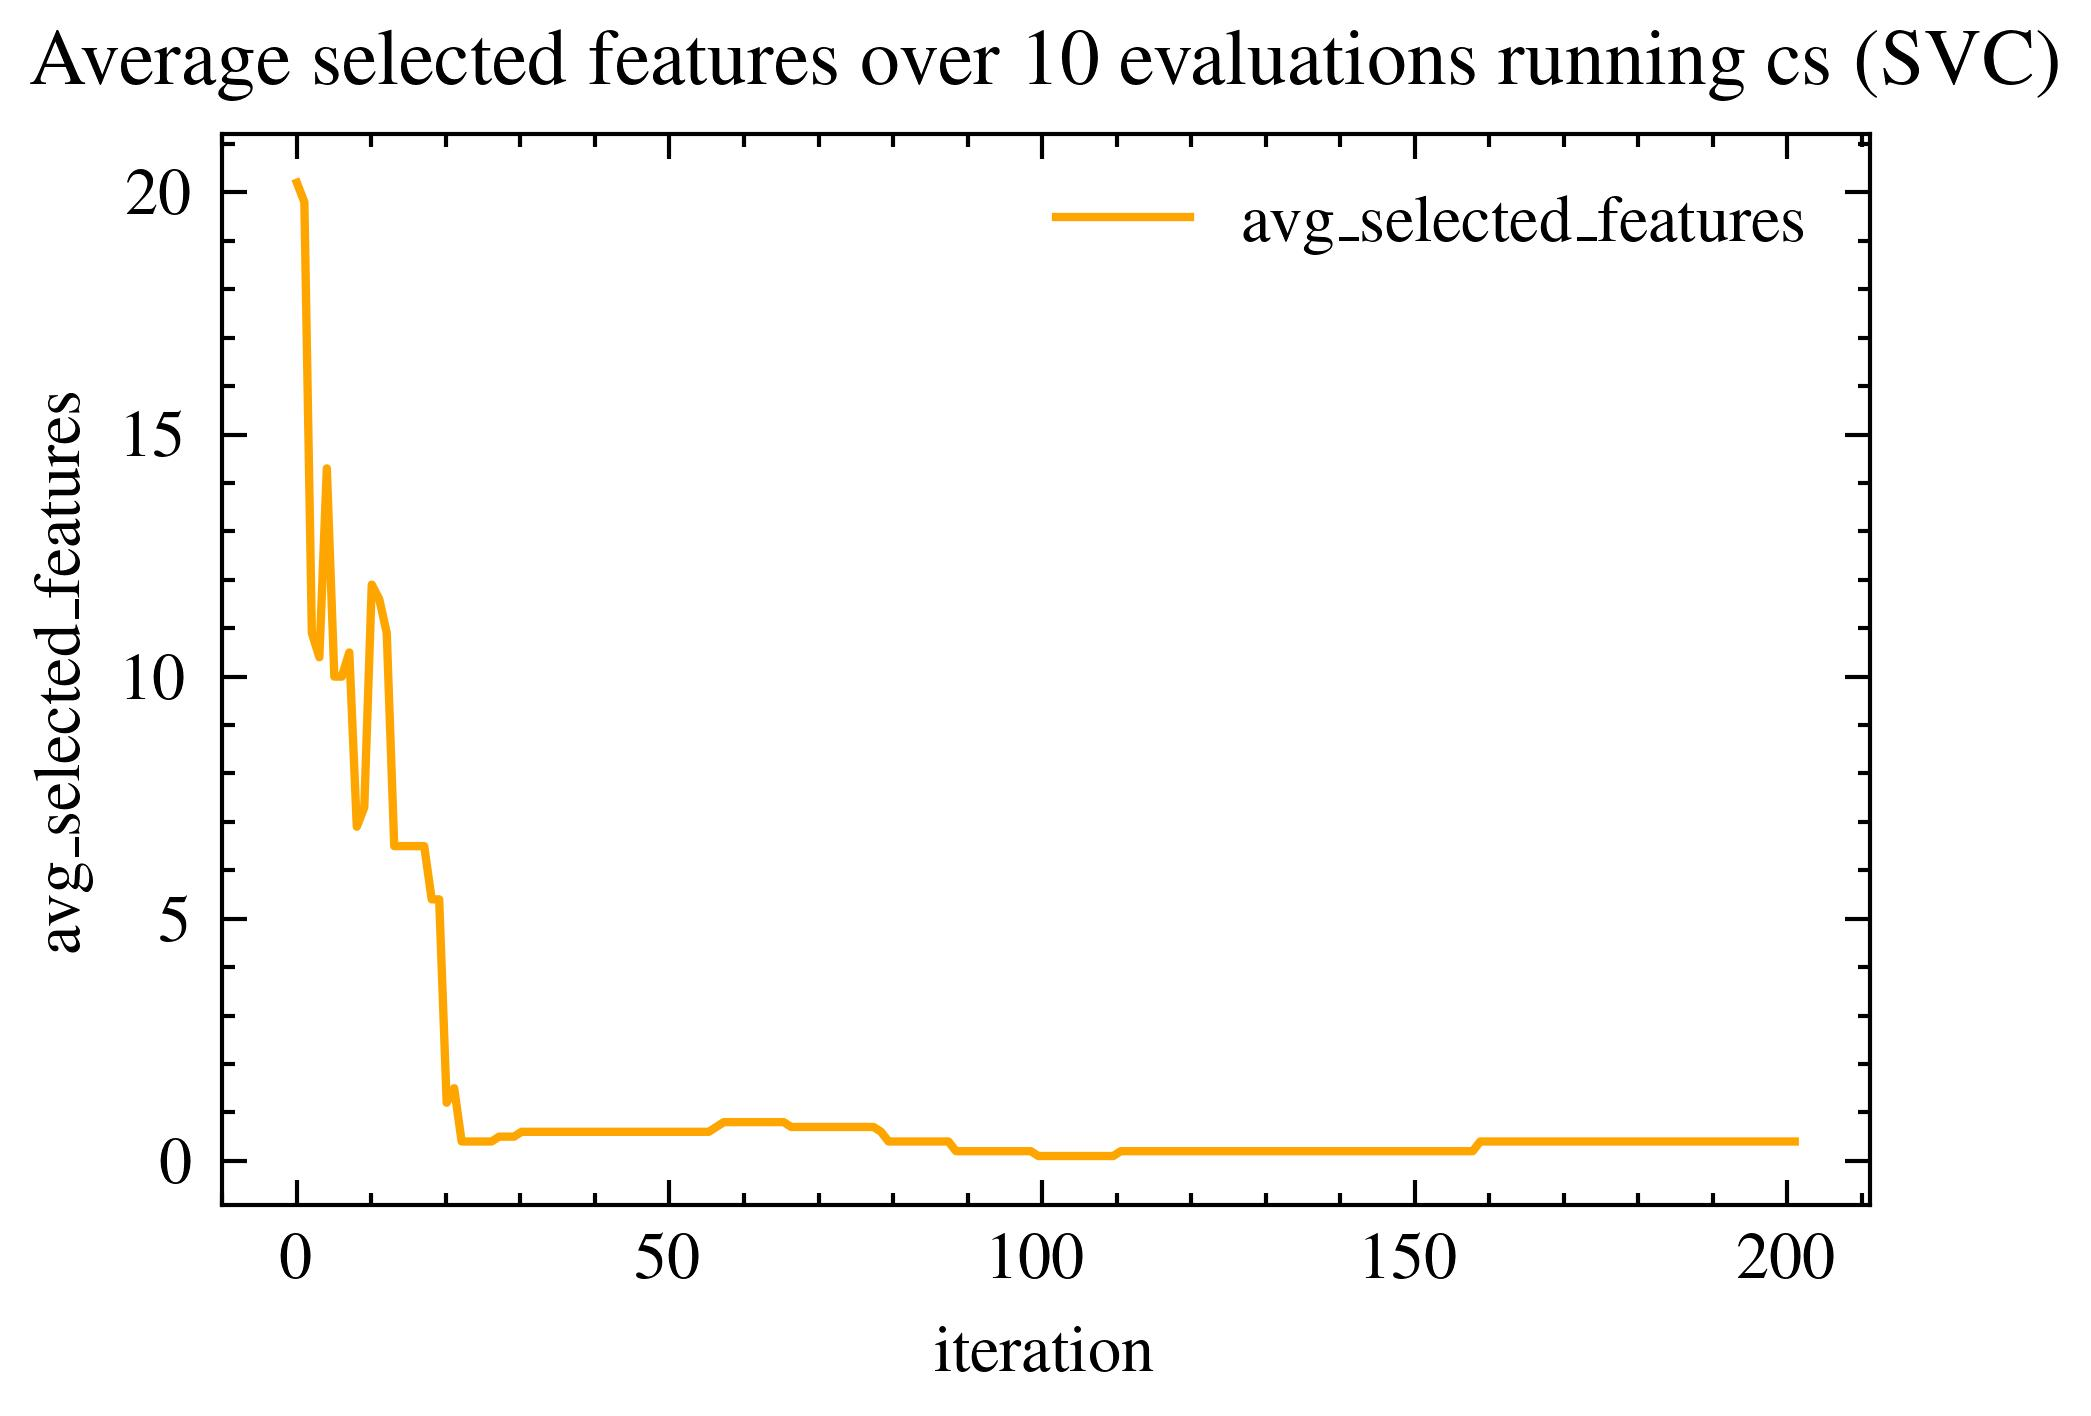
\includegraphics[width=\textwidth]{imagenes/fitness_charts/img/real/spectf-heart/SVC_n_features_over_10_evaluations_cs_real_spectf-heart.jpg}
        \caption{spectf-heart}
    \end{subfigure}
    \begin{subfigure}[htp]{0.45\textwidth}
        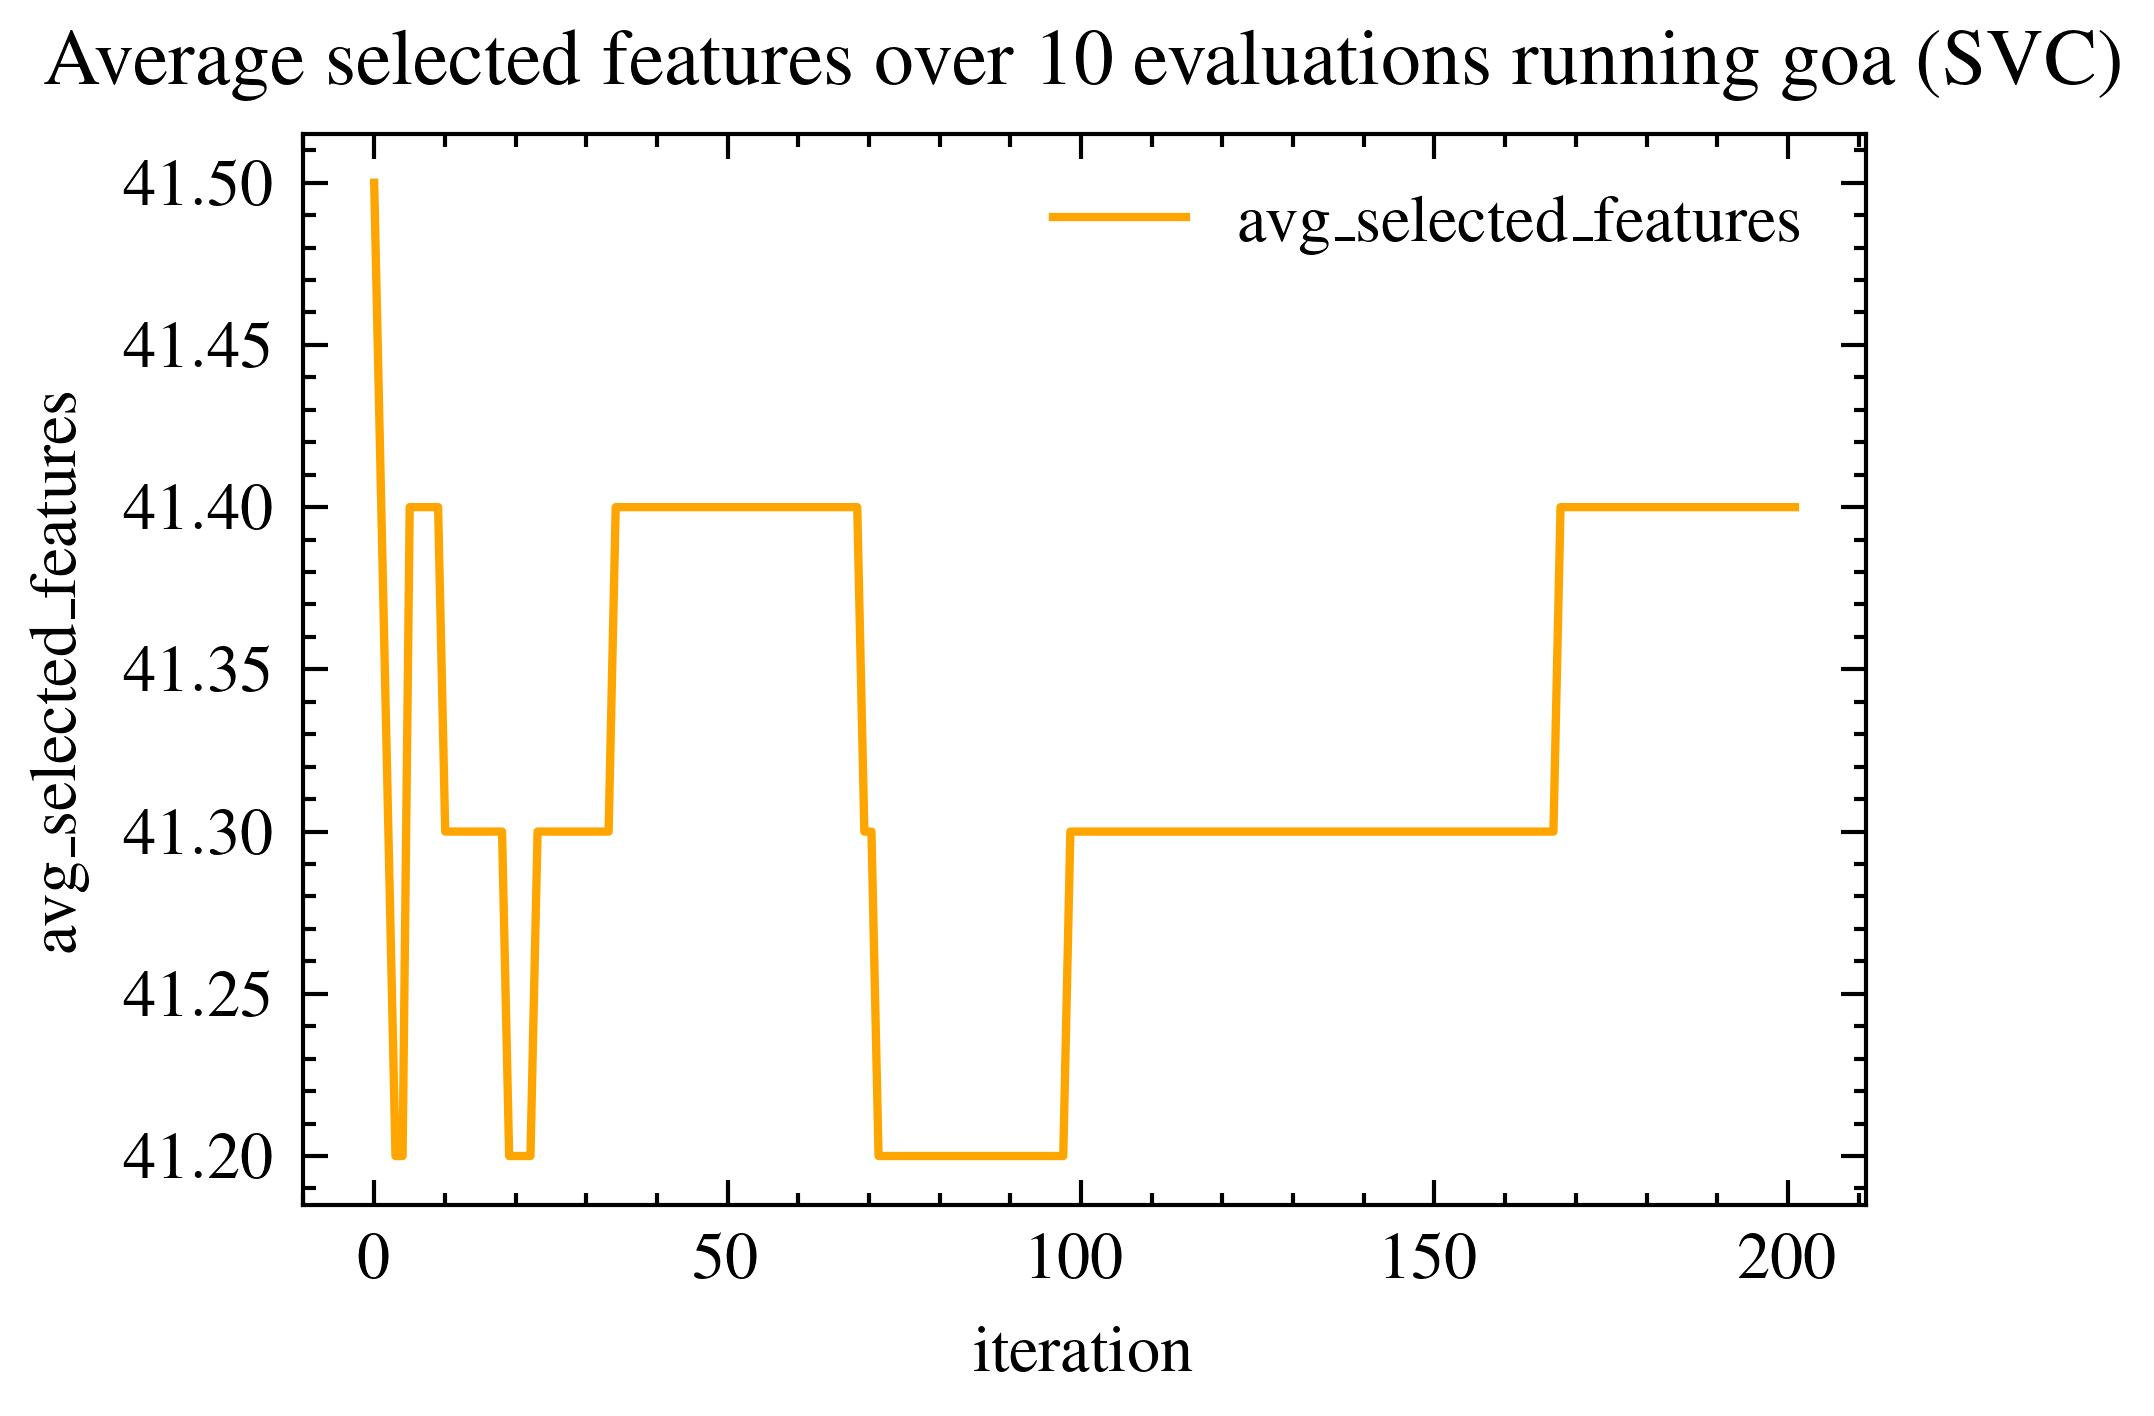
\includegraphics[width=\textwidth]{imagenes/fitness_charts/img/real/spectf-heart/SVC_n_features_over_10_evaluations_goa_real_spectf-heart.jpg}
        \caption{spectf-heart}
    \end{subfigure}

    \begin{subfigure}[htp]{0.45\textwidth}
        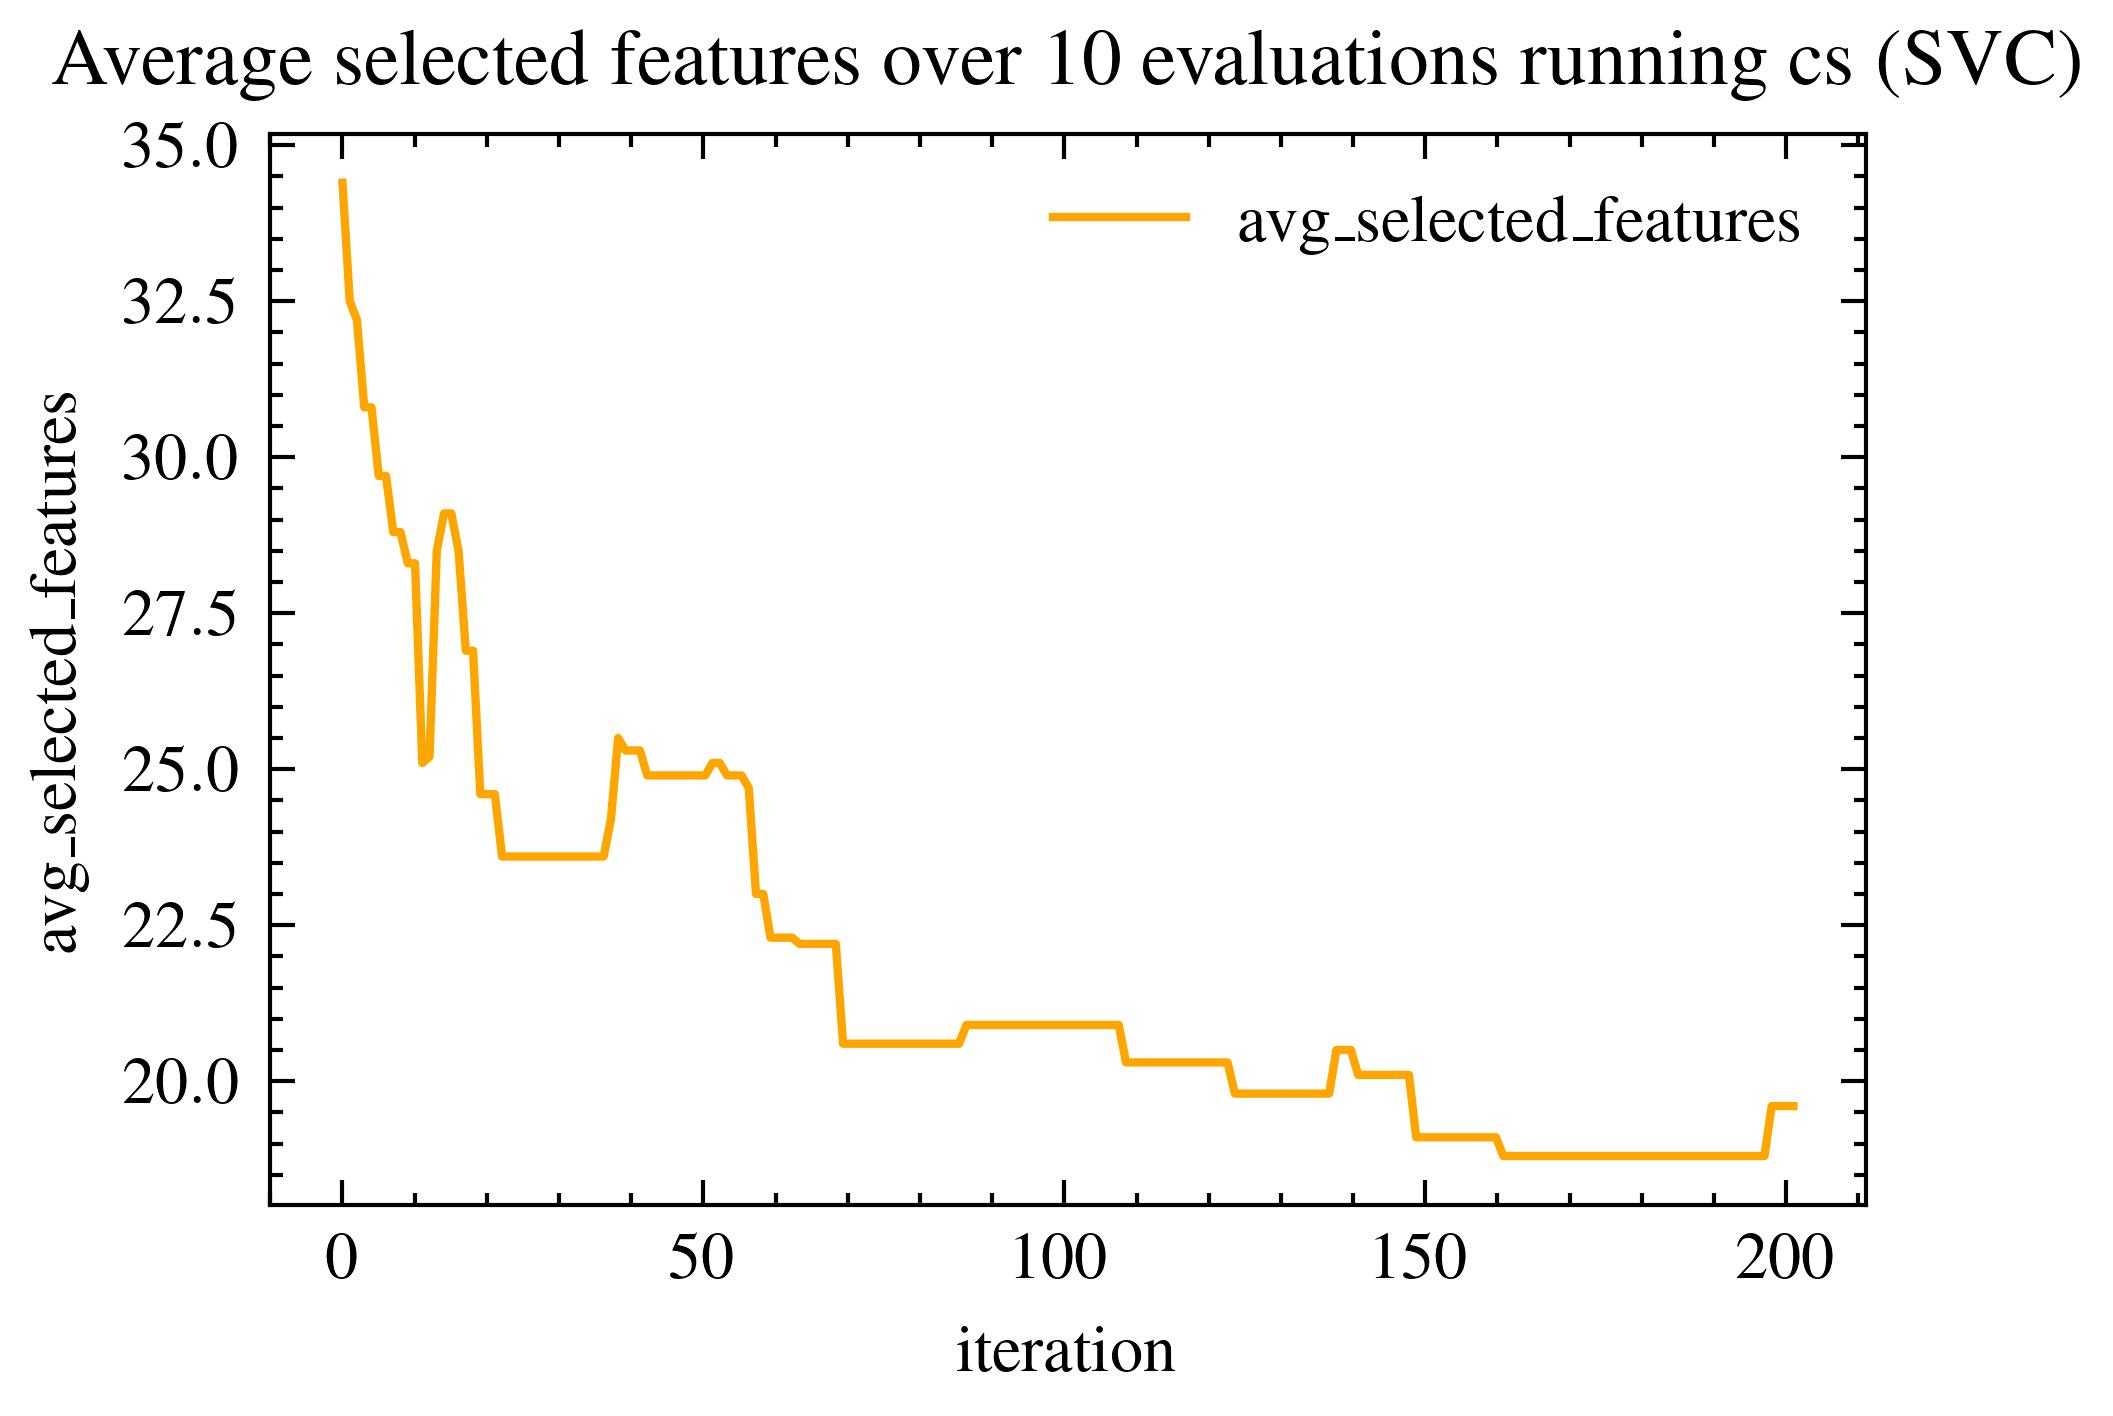
\includegraphics[width=\textwidth]{imagenes/fitness_charts/img/real/waveform5000/SVC_n_features_over_10_evaluations_cs_real_waveform5000.jpg}
        \caption{waveform5000}
    \end{subfigure}
    \begin{subfigure}[htp]{0.45\textwidth}
        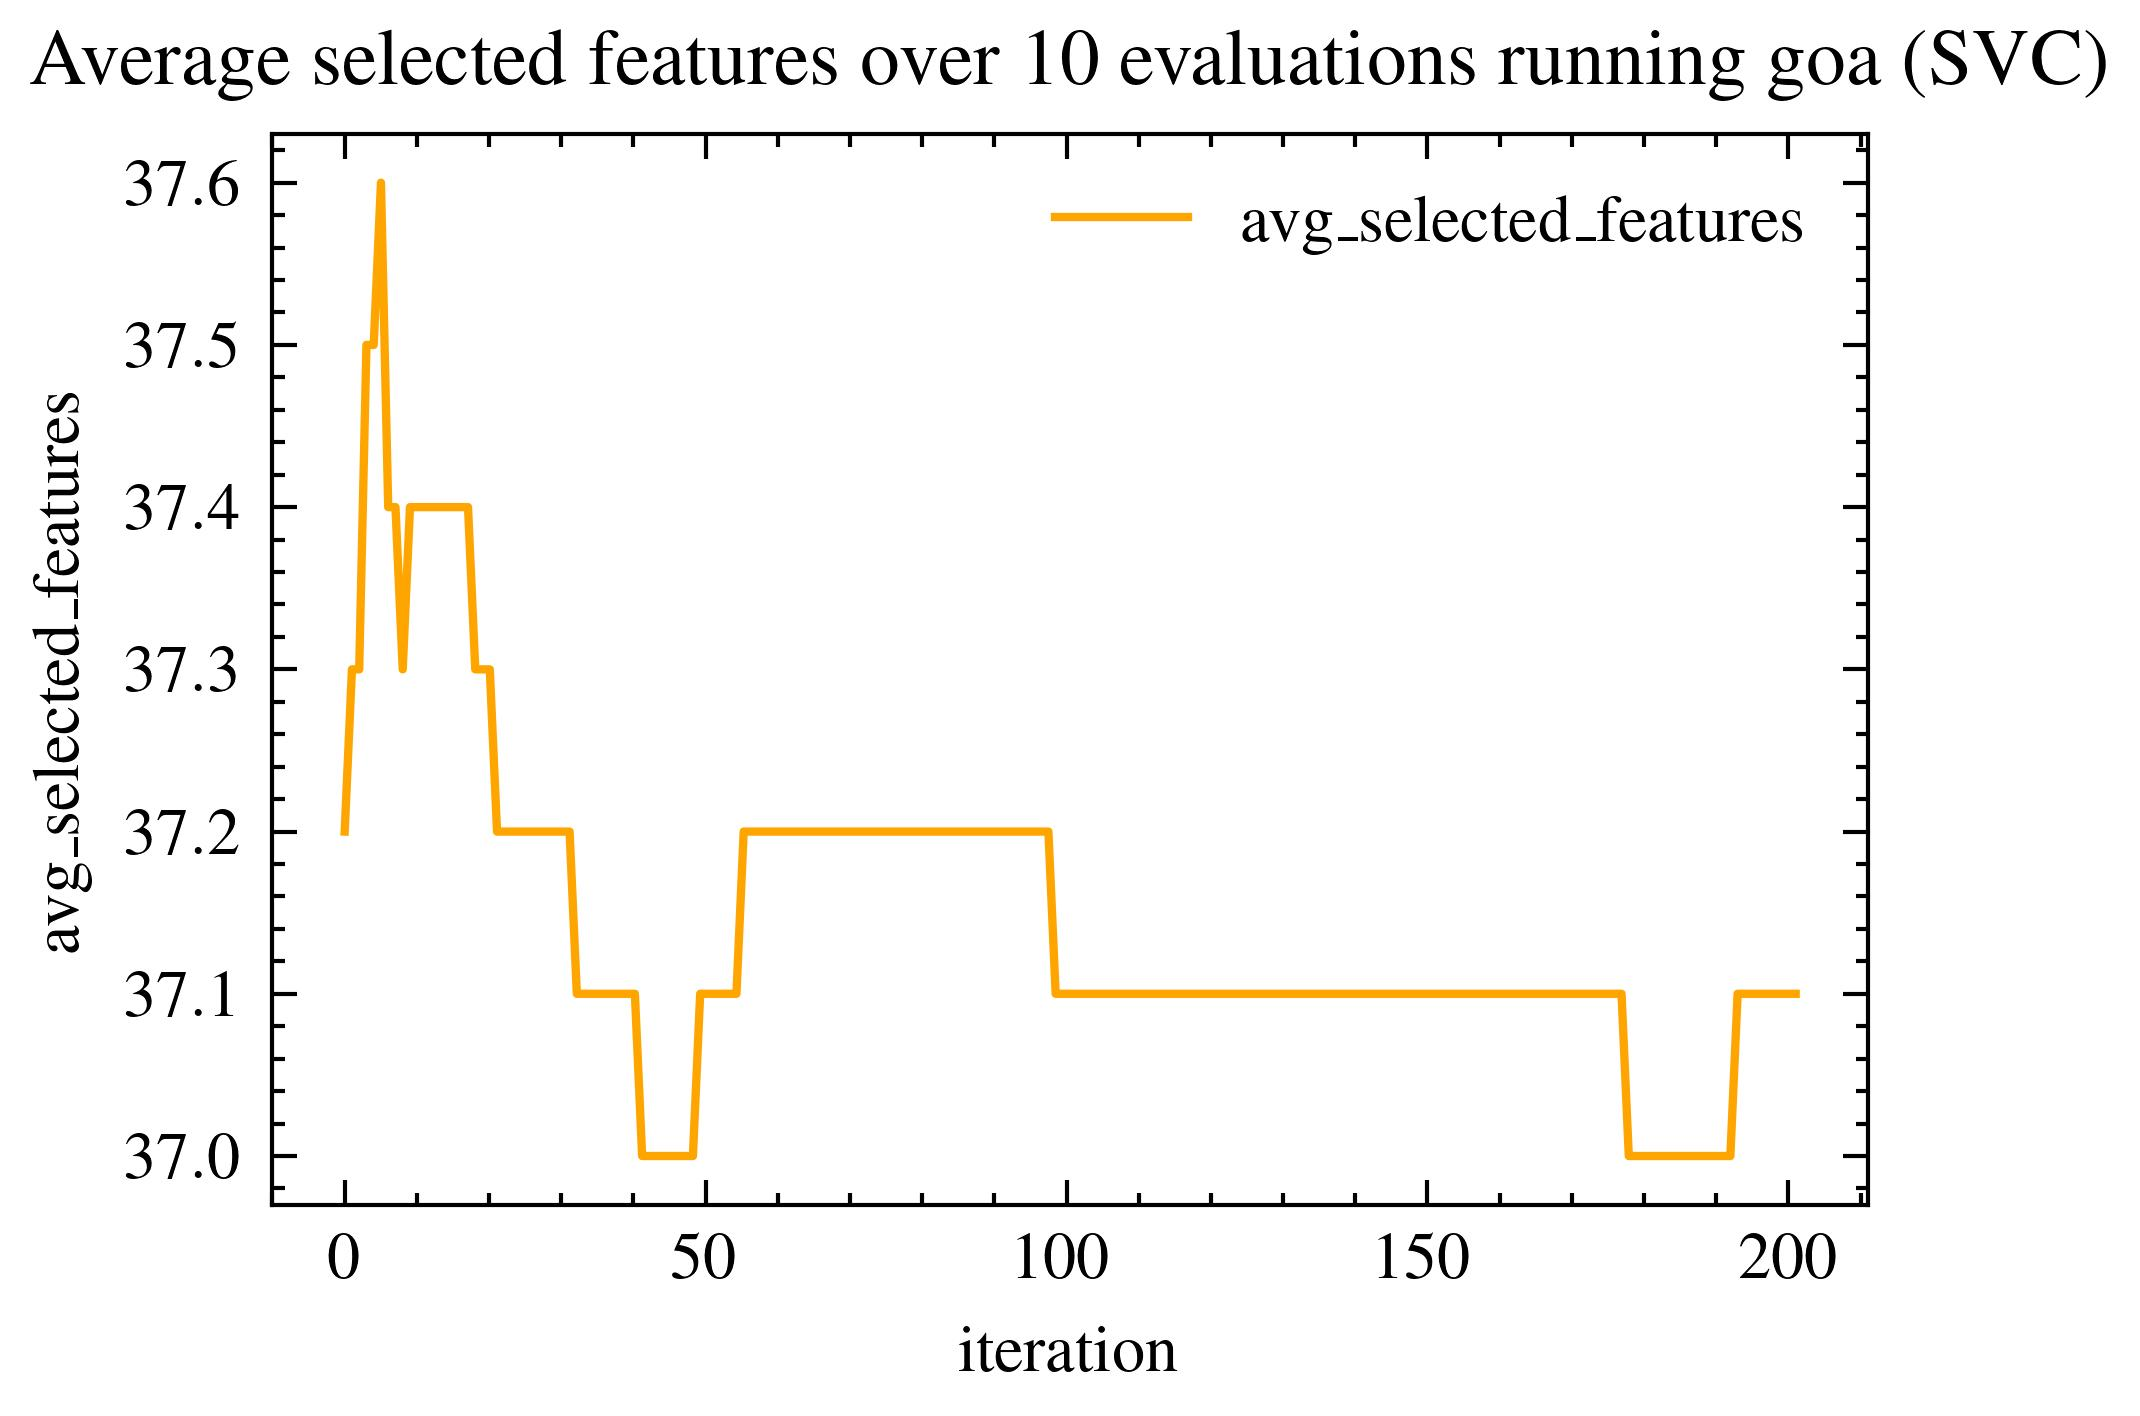
\includegraphics[width=\textwidth]{imagenes/fitness_charts/img/real/waveform5000/SVC_n_features_over_10_evaluations_goa_real_waveform5000.jpg}
        \caption{waveform5000}
    \end{subfigure}

    \begin{subfigure}[htp]{0.45\textwidth}
        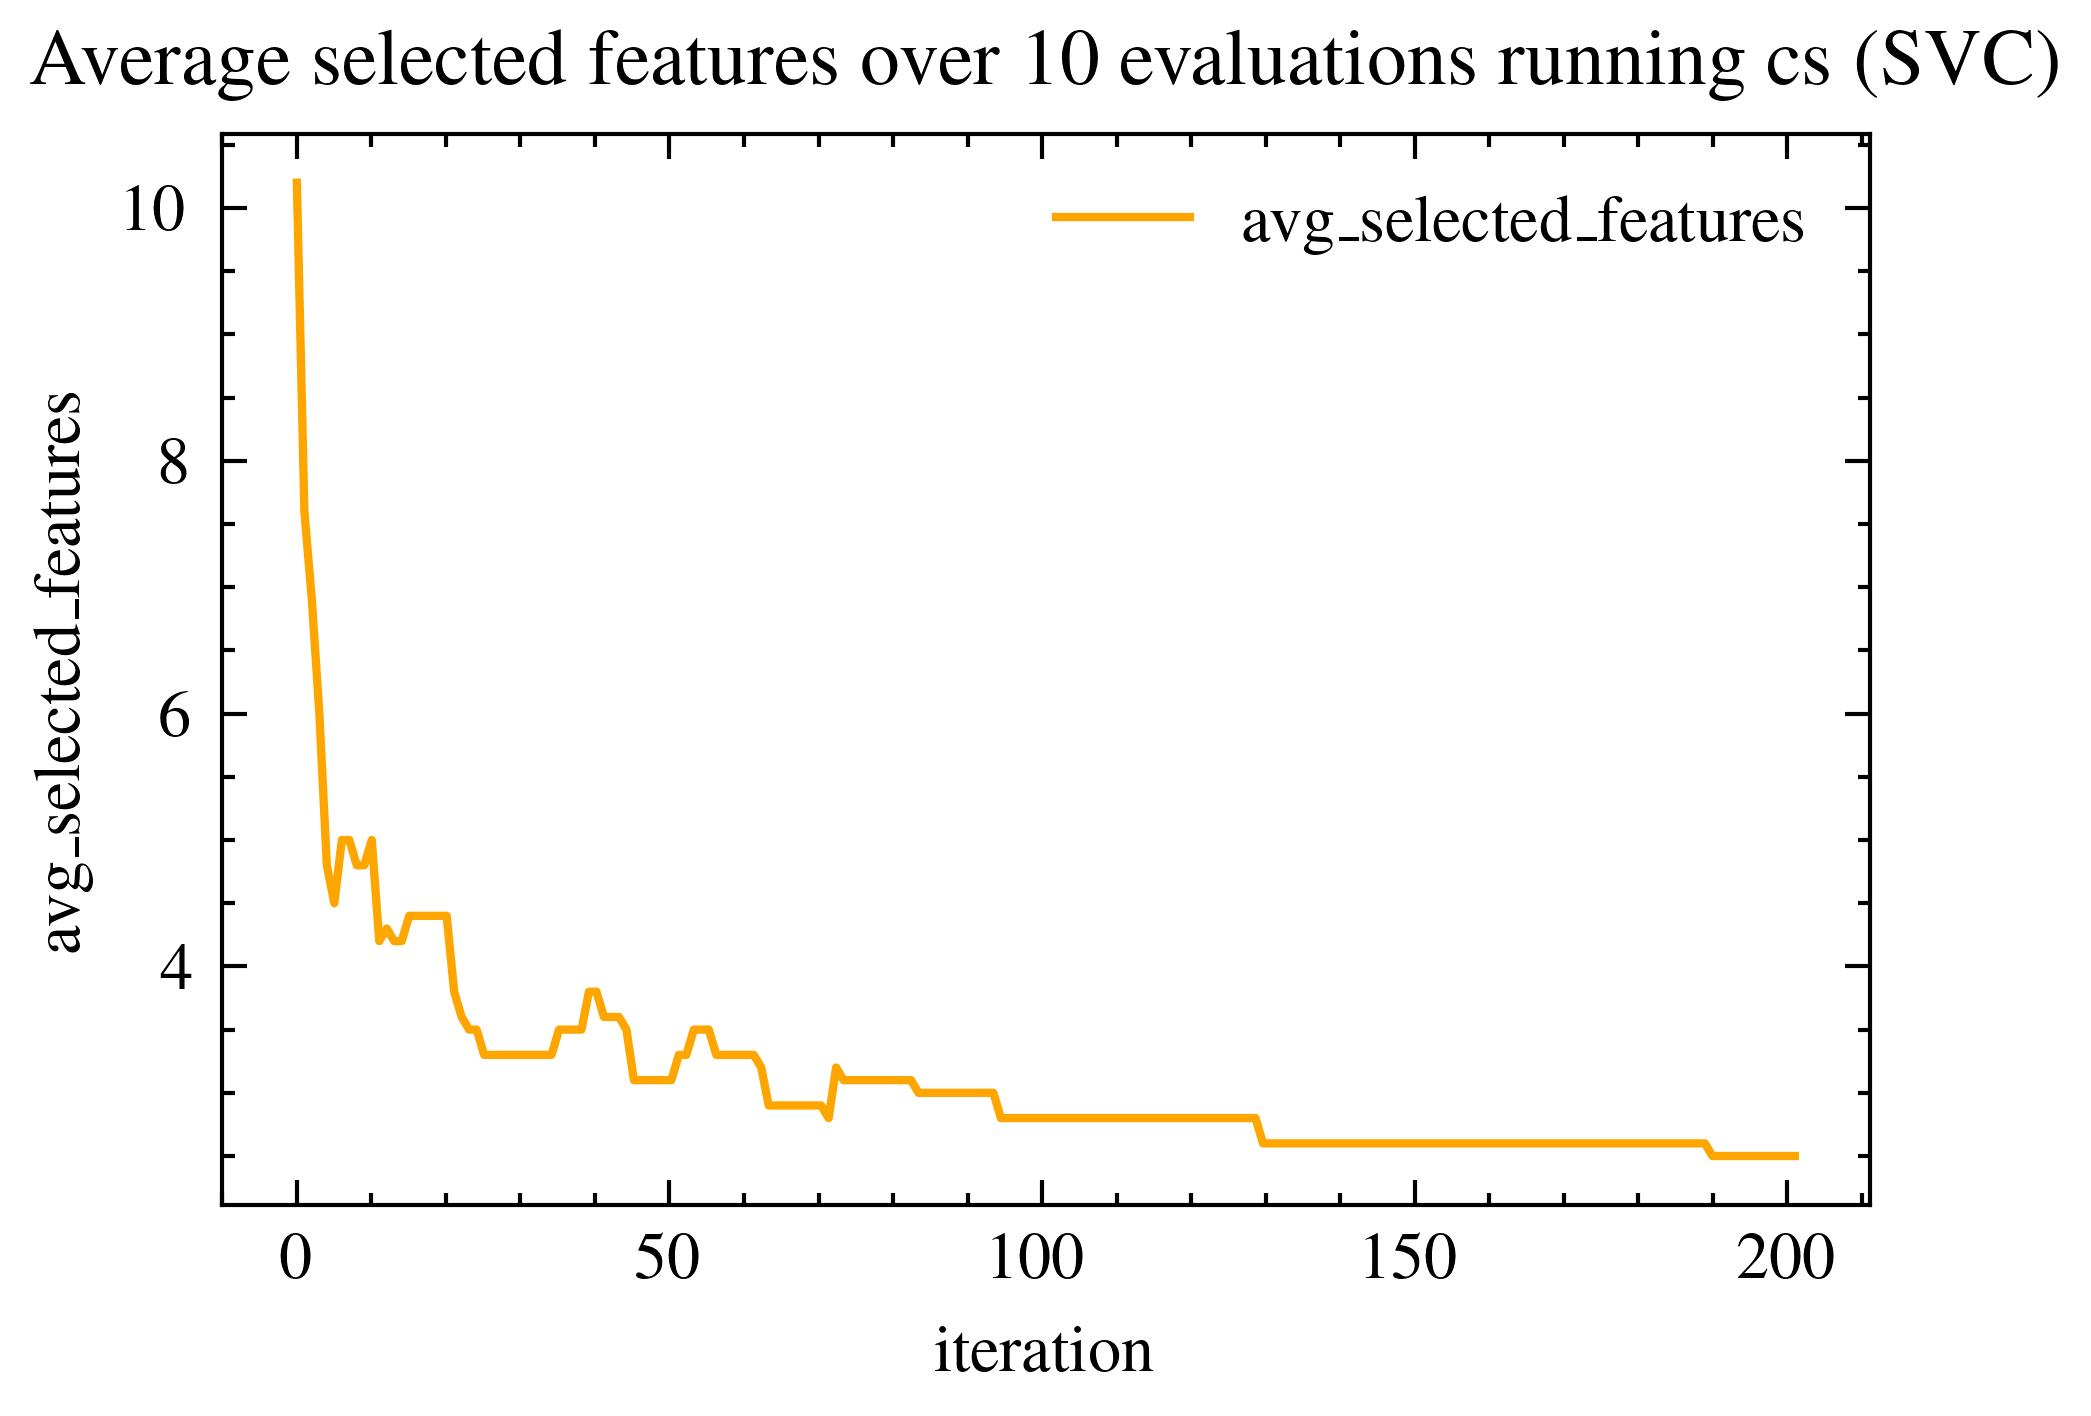
\includegraphics[width=\textwidth]{imagenes/fitness_charts/img/real/wine/SVC_n_features_over_10_evaluations_cs_real_wine.jpg}
        \caption{wine}
    \end{subfigure}
    \begin{subfigure}[htp]{0.45\textwidth}
        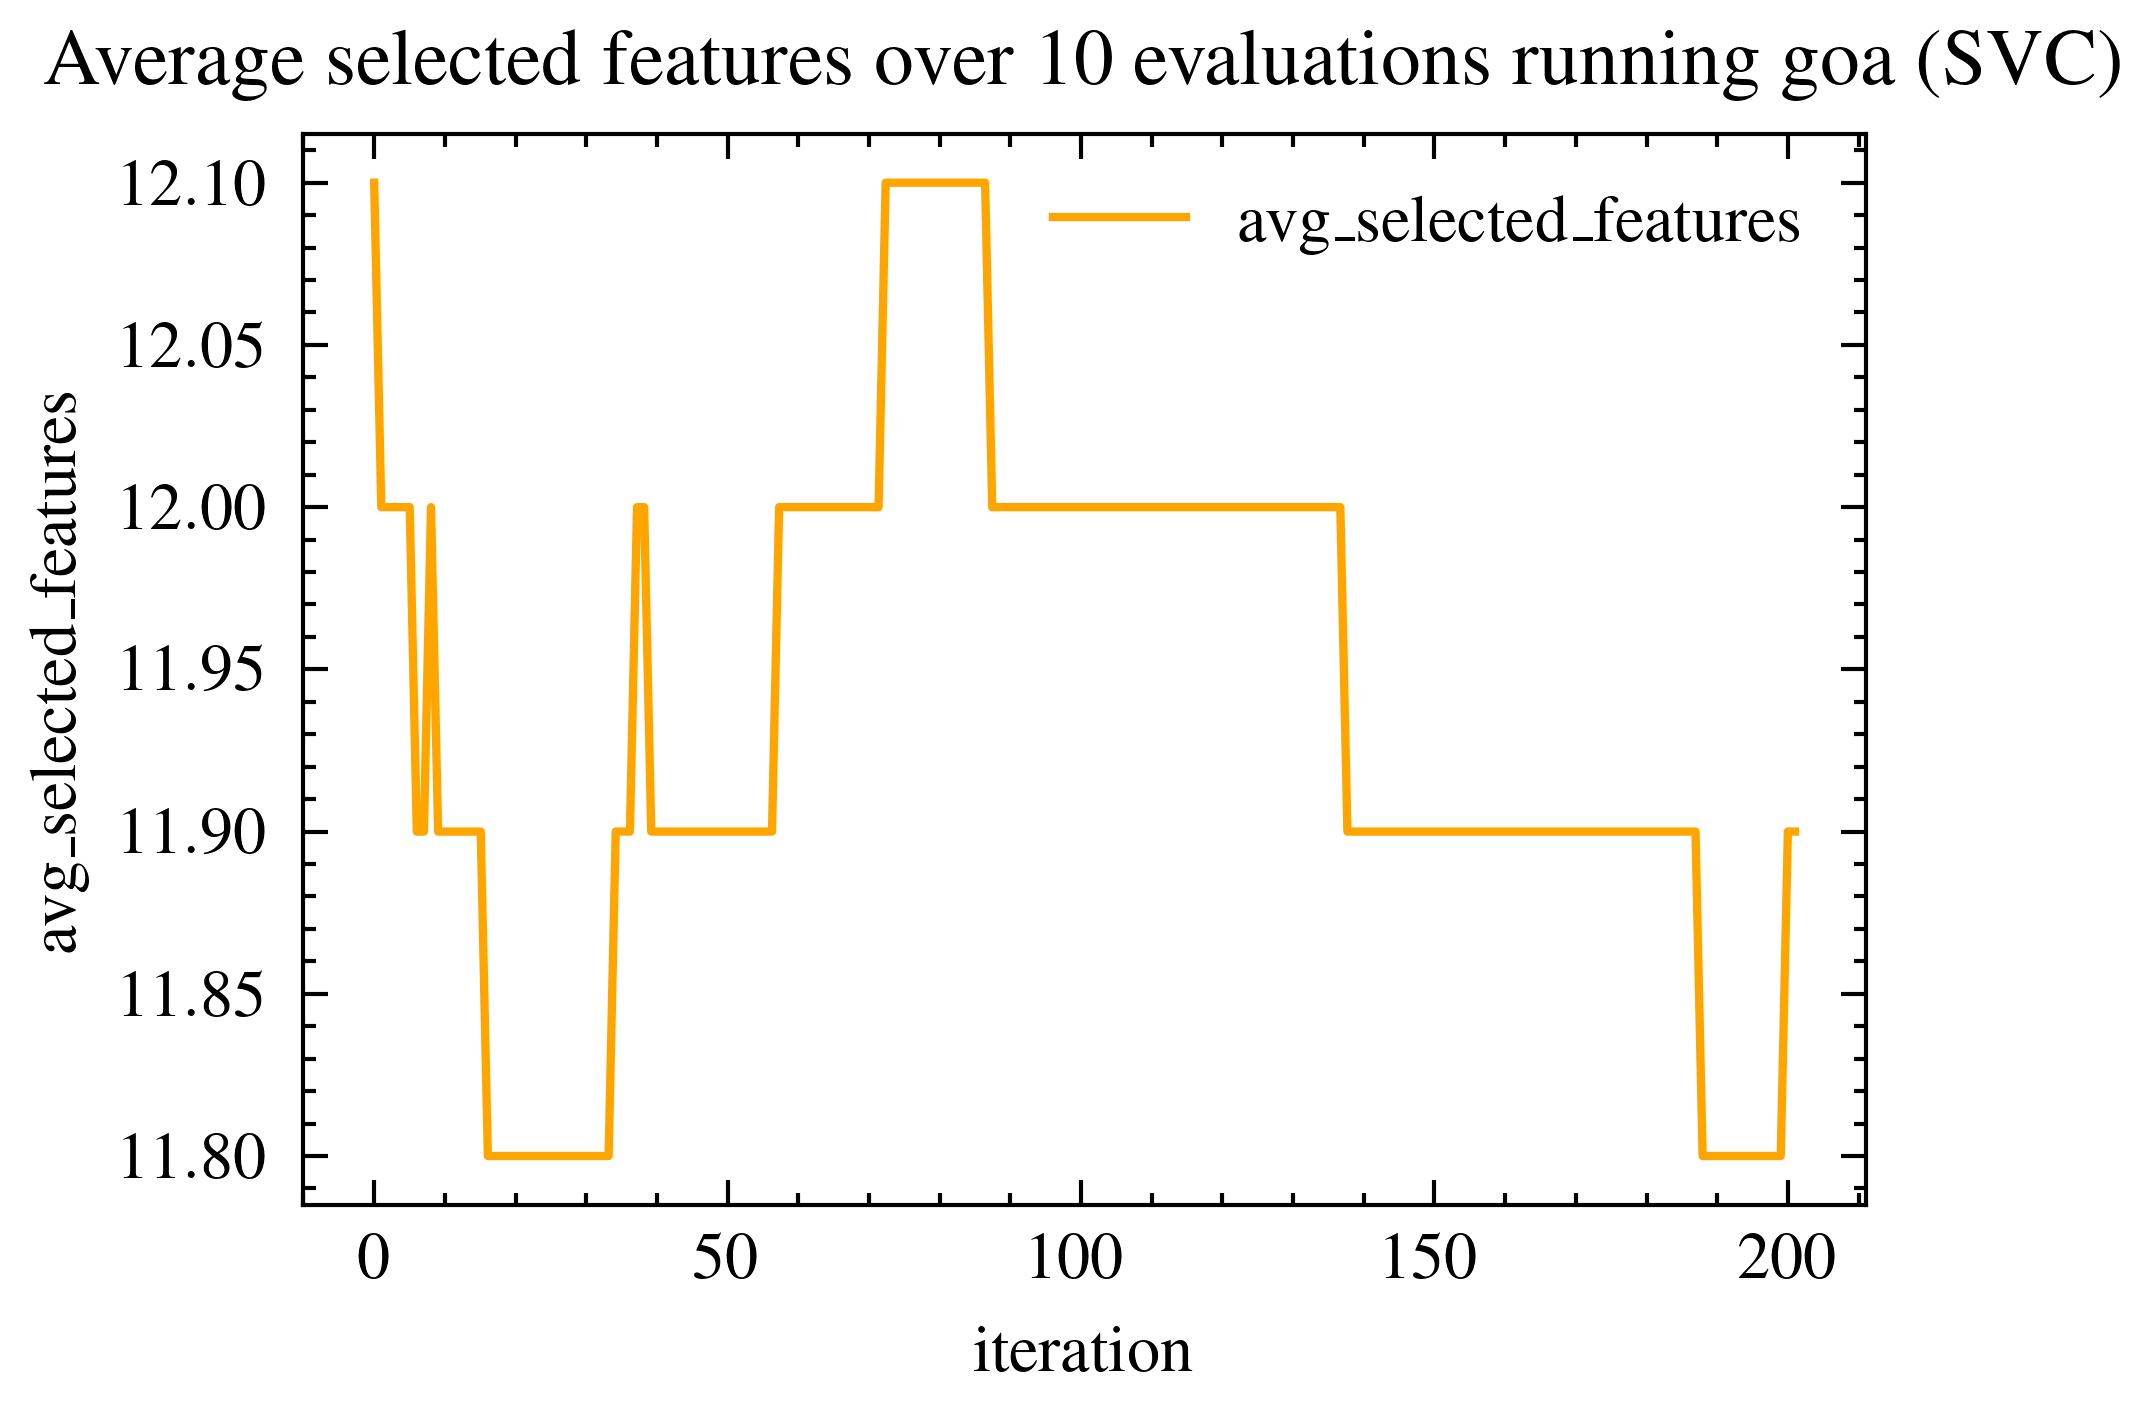
\includegraphics[width=\textwidth]{imagenes/fitness_charts/img/real/wine/SVC_n_features_over_10_evaluations_goa_real_wine.jpg}
        \caption{wine}
    \end{subfigure}
    \caption{Reducción de características en CS y GOA}
    \label{fig:svc_selected_rate_cs_goa_real}
\end{figure}

En las figuras \ref{fig:svc_selected_rate_cs_goa_real} se puede apreciar la mejora de la reducción de características con el tiempo entre algunos \textit{datasets} para \textbf{CS} y \textbf{GOA}. Como puede observarse, la diferencia es bastante grande. De hecho, se puede apreciar en la escala del \textbf{GOA}, que este apenas reduce, de hecho, a veces aumenta la cantidad de atributos elegidos. Dados estos resultados tan desfavorables para \textbf{GOA}, es obvio ver que estos no son dados por el azar casi con toda seguridad. Pese a ello se adjunta tabla con p-valores confirmando lo evidente en \ref{tab:pval_corr_best-worst-real_svc_knn}.

\begin{table}
    \centering
    \begin{tabular}{lll}
        \toprule
        {}  & cs                     & goa                    \\
        \midrule
        cs  & -                      & - (\textbf{6.104E-05}) \\
        goa & + (\textbf{6.104E-05}) & -                      \\
        \bottomrule
    \end{tabular}
    \caption{P-valores tras corrección entre CS y GOA - knn y svc - real}
    \label{tab:pval_corr_best-worst-real_svc_knn}
\end{table}

\subsubsection{Clásicos vs Modernos}
Como se destacó previamente, las diferencias de \textit{accuracy} entre los algoritmos son minúsculas, por lo que no hay apenas diferencias entre los dos grupos. La característica más discriminatoria es la reducción de características y se puede observar en los rankings qué algoritmos ponderan mejor y peor (\ref{tab:ranking_sel_rate_real_svc}, \ref{tab:ranking_sel_rate_real_knn}).\\[6pt]
De nuevo como en la comparación del fitness, se obtienen puestos promedios para el grupo de algoritmos clásicos, por lo que son capaces de reducir incluso en su versión continua, pero los que más destacan son un subgrupo de algoritmos modernos. Igualmente, si comparamos las pocas diferencias que se encuentran en \textit{accuracy} en los rankings de \ref{tab:ranking_accuracy_real_knn} y \ref{tab:ranking_accuracy_real_svc}, se puede ver como los clásicos adelantan en posición a \textbf{WOA} y \textbf{BA} en \textbf{SVC} y mejoran puestos en \textbf{kNN}. Es decir, los algoritmos clásicos obtienen mejor precisión (solo un poco), pero reducen menos, según los resultados recogidos.\\[6pt]
Aunque la tendencia parezca esta, las diferencias son nimias y por tanto no hay ninguna mejora significativa en cuanto a \textit{accuracy}. Si hay diferencias significativas en reducción de características entre algoritmos de distintas posiciones, pero ocurre tanto para clásicos como para modernos. Por ello, dependiendo del balance entre \textit{accuracy} y reducción de características  deseado dependerá de la problemática tratada. Los clásicos parecen una opción segura por los buenos resultados obtenidos en \textit{accuracy} y los resultados promedio en reducción dimensional. Si se requieren reducciones más extremas de las dimensiones de un conjunto de datos, quizá cierta selección de modernos pueda ser aplicada con mayor éxito.